\documentclass[12pt]{uthesis-v12}  %---> DO NOT ALTER THIS COMMAND

\usepackage{graphicx}
\usepackage{amssymb}
\usepackage{algorithm2e}
\usepackage{algpseudocode}

\begin{document} %---> %---> %---> %---> DO NOT ALTER THIS COMMAND
%--------+----------------------------------------------------------+
%        |  \title{}                                    (REQUIRED)  |
%        |  \author{}                                   (REQUIRED)  |
%        |                                                          |
%        |  See section 3.1 of "Read_Me_First_(v12).pdf"            |
%        |                                                          |
%        |  Also see section 2.2 of above "Read Me" file for the    |
%        |  proper use of the invisible tilde ("~") character when  |
%        |  entering a middle initial in the \author command.       |
%        +----------------------------------------------------------+

\title{Optimizing Android Memory Management
       \protect\\ by Predicting User Behavior}
       
% Alternatively, A User-Centric Approach to Android Memory Management

\author{Srinivas Muthu}

%--------+----------------------------------------------------------+
%        |  \copyrightpage{}                            (REQUIRED)  |
%        |                                                          |
%        |  See section 3.2 of "Read_Me_First_(v12).pdf"            |
%        |                                                          |
%        |  1) You must enter either "yes" or "no" in this          |
%        |      command.  Inputting "yes" produces a copyright      |
%        |      notification page as the second page and inputting  |
%        |      "no" produces a blank second page.                  |
%        |  2) Input to this command is case sensitive.             |
%        |  3) Default: the "yes" option.                           |
%        +----------------------------------------------------------+

\copyrightpage{yes}

%--------+----------------------------------------------------------+
%        |  \mydocument{}                               (REQUIRED)  |
%        |                                                          |
%        |  See section 3.3 of "Read_Me_First_(v12).pdf"            |
%        |                                                          |
%        |  1) Input to this command is limited to the following    |
%        |     three options: a) Dissertation                       |
%        |                    b) Thesis                             |
%        |                    c) Project                            |
%        |  2) Input to this command is case-sensitive.             |
%        +----------------------------------------------------------+

\mydocument{Thesis}

%--------+----------------------------------------------------------+
%        |  \degree{}{}                                 (REQUIRED)  |
%        |                                                          |
%        |  See section 3.4 of "Read_Me_First_(v12).pdf"            |
%        |                                                          |
%        |  You need to provide two distinct inputs into this       |
%        |  command:                                                |
%        |     1) In the first set of braces you need to specify    |
%        |        the *exact* degree you will receive. Some         |
%        |        examples are: -) Masters of Arts                  |
%        |                      -) Masters of Science               |
%        |                      -) Doctor of Philosophy             |
%        |     2) In the second set of braces you need to state the |
%        |        *specific* discipline or area for that degree     |
%        |        (e.g., Economics, Education, Engineering, etc.).  |
%        |  Students should consult their advisor if they have any  |
%        |  questions about this information.                       |
%        +----------------------------------------------------------+

\degree{Masters of Science}{Engineering}

%--------+----------------------------------------------------------+
%        |  \conferraldate{}{}                          (REQUIRED)  |
%        |                                                          |
%        |  See section 3.5 of "Read_Me_First_(v12).pdf"            |
%        |                                                          |
%        |  In the two set of braces enter the month and then the   |
%        |  year your degree will be *conferred* by the university. |
%        +----------------------------------------------------------+

\conferraldate{December}{2015}

%--------+----------------------------------------------------------+
%        |  \advisor{}                                  (REQUIRED)  |
%        |                                                          |
%        |  See section 3.6.2 of "Read_Me_First_(v12).pdf"          |
%        |                                                          |
%        |  1) Also see section 2.2 of "Read_Me_First_(v12).pdf"    |
%        |     for the proper use of the invisible tilde ("~")      |
%        |     character when entering a middle initial or the      |
%        |     abbreviation of an academic title (e.g., Dr.) in     |
%        |     the \advisor{} command.                              |
%        |  2) Also see section 3.6.1. for consistent presentation  |
%        |     of title page signature lines.                       |
%        +----------------------------------------------------------+

\advisor{Dr.~Jackson Carvalho}

%--------+----------------------------------------------------------+
%        |  Committee Member Signature Commands         (OPTIONAL)  |
%        |                                                          |
%        |  See section 3.6.3 of "Read_Me_First_(v12).pdf"          |
%        |                                                          |
%        |  1) Use the commands below to provide signature lines    |
%        |     for your "other" committee members;                  |
%        |        --> you must list your other committee members    |
%        |            in alphabetic order by last name              |
%        |        --> to do this, use the commands below in the     |
%        |            order presented below.                        |
%        |  2) You can choose to include none, some, or all of the  |
%        |     "XXXmember" commands below --- based on the number   |
%        |     committee members you have; simply delete (or        |
%        |     comment-out) any of the commands below that are not  |
%        |     needed.                                              |
%        |  3) Do not include the name of your committee chair or   |
%        |     the Graduate Dean in the commands listed below.      |
%        |     Their signature lines are generated by the           |
%        |     \advisor{} and \graduatedean{}{} commands.           |
%        |  4) You cannot use any of the commands below more than   |
%        |     once. (For details on this issue, see section 3.6.3  |
%        |     of "Read_Me_First_(v12).pdf".)                       |
%        |  5) Also see section 2.2 of "Read_Me_First_(v12).pdf"    |
%        |     for the proper use of the invisible tilde ("~")      |
%        |     character when entering a middle initial or the      |
%        |     abbreviation of an academic title (e.g., Dr.) in     |
%        |     the commands below.                                  |
%        |  6) See section 3.6.1. for consistent presentation of    |
%        |     title page signature lines.                          |
%        |                                                          |
%        |  I know I shouldn't have to say this, but enough         |
%        |  students over the years have made the same mistake      |
%        |  that I'm forced to state:                               |
%        |                                                          |
%        |      THE NAMES USED IN THE FOLLOWING COMMANDS ARE        |
%        |      SILLY NAMES I'VE USED AS EXAMPLES ONLY.  THEY       |
%        |      ARE NOT THE ACTUAL NAMES OF YOUR COMMITTEE          |
%        |      MEMBERS.  REPLACE THE SILLY NAMES BELOW WITH        |
%        |      THE NAMES OF YOUR ACTUAL COMMITTEE MEMBERS.         |
%        |                                                          |
%        +----------------------------------------------------------+

  \secondmember{Dr.~Mansoor Alam}
   \thirdmember{Dr.~Henry Ledgard}

%--------+----------------------------------------------------------+
%        |  \graduatedean{}{}                           (REQUIRED)  |
%        |                                                          |
%        |  See section 3.6.4 of "Read_Me_First_(v12).pdf"          |
%        |                                                          |
%        |  1) THE NAME AND TITLE PROVIDED BELOW ARE THOSE OF THE   |
%        |     ACTUAL GRADUATE DEAN AT THE TIME THIS DOCUMENT WAS   |
%        |     CONSTRUCTED (January 2012). Contact the Graduate     |
%        |     College to determine whether this information is     |
%        |     correct at the time you submit your document.        |
%        |  2) Section 2.2 of "Read_Me_First_(v12).pdf" describes   |
%        |     the proper use of the invisible tilde ("~")          |
%        |     character when entering a middle initial or the      |
%        |     abbreviation of an academic title (e.g., Dr.) in     |
%        |     the \graduatedean{} command.                         |
%        |  3) See section 3.6.1. for consistent presentation of    |
%        |     title page signature lines.                          |
%        +----------------------------------------------------------+

\graduatedean{Dr.~Patricia R.~Komuniecki}{Dean}

%--------+----------------------------------------------------------+
%        |  \maketitle                                  (REQUIRED)  |
%        |                                                          |
%        |  See section 3.7 of "Read_Me_First_(v12).pdf"            |
%        |                                                          |
%        |  This is a required LaTeX command; to be brief, bad      |
%        |  things will happen if this command is not included      |
%        |  in your document at this particular location.           |
%        +----------------------------------------------------------+

\maketitle  %---->  ----->  ---->  ---->   DO NOT ALTER THIS COMMAND

%--------+----------------------------------------------------------+
%        |  Abstract Page Environment                   (REQUIRED)  |
%        |                                                          |
%        |  See section 3.8 of "Read_Me_First_(v12).pdf"            |
%        +----------------------------------------------------------+

\begin{abstractpage}
With the advent of increase in the amount of RAM (Random Access memory) available in Android smart-phones, there is a case to be made that this additional memory availability can be put to better use. By default, every Android application runs in its own Linux process. When a smart-phone that runs on Android is active, the RAM contains all the active processes and services (processes that run in the background). In addition to these processes and services, the RAM also contains cached background processes. These processes are kept in memory so that in the event the user clicks any of the corresponding applications, they can be loaded onto the screen quickly. If Android needs to reclaim memory for other processes, it eliminates cached background processes through an LRU (Least Recently Used) scheme. We postulate that analyzing  user behavior could help us better determine which applications to cache in memory, as cached background processes. We parse the user's Calendar for contextual clues and gather information that could help us predict which application a user is about to use. We measure the cache efficiency (Cache hits and misses, CHR (Cache Hit Ratio)) for the default CRA (Cache Replacement Algorithm) Android employs (LRU), a pure prediction based CRA and finally a hybrid approach that combines the LRU approach with the prediction approach. We also demonstrate why the hybrid CRA is the most efficient one.


\end{abstractpage}

%--------+----------------------------------------------------------+
%        |  Dedication Page Environment                 (OPTIONAL)  |
%        |                                                          |
%        |  See section 3.9 of "Read_Me_First_(v12).pdf"            |
%        |                                                          |
%        |  If both a dedication page and an acknowledgements page  |
%        |  are included in the document, the dedication page must  |
%        |  proceed the acknowledgements page.                      |
%        +----------------------------------------------------------+

\begin{dedication}
\noindent To my parents who've always put my needs ahead of theirs.
\end{dedication}

%--------+----------------------------------------------------------+
%        |  Acknowledgments Page Environment            (OPTIONAL)  |
%        |                                                          |
%        |  See section 3.10 of "Read_Me_First_(v12).pdf"           |
%        |                                                          |
%        |  If both a dedication page and an acknowledgements page  |
%        |  are included in the document, the dedication page must  |
%        |  proceed the acknowledgements page.                      |
%        +----------------------------------------------------------+

\begin{acknowledgments}
\noindent First and foremost, I'd like to thank Dr.~Jackson Carvalho for mentoring me throughout my time here at UT. Without his guidance, I would'nt be half the student I am today. I'd like to thank Dr.~Mansoor Alam for believing in me and offering me tuition scholarship to pursue graduate studies, here at UT. I'd like to thank Dr.~Lawrence Thomas for being an exemplary professor and his words of wisdom have always guided me in tough times.\\\\I am grateful to Dr.~Henry Ledgard for taking the time to be on my committee and mentoring me during my freshman year. I'd like to thank Dr.~Donald White and his students for helping me with data collection, design and representation. It was nothing short of a privelege to work with Dr.~White and his students. I'd like to thank Dean Nagi G.~Naganathan for employing me and guiding me over the course of my time in graduate school.\\\\
I'd like to thank all my friends and family for supporting me throughout my time here at UT but I'd like to especially mention Sandy Stewart for everything she's done for me. This page is'nt enough to expound on the details but it suffices to say I would'nt be here without her and she is like a second mother to me.  
\end{acknowledgments}

%--------+----------------------------------------------------------+
%        |  \tableofcontents                            (REQUIRED)  |
%        |  \listoftables                            (CONDITIONAL)  |
%        |  \listoffigures                           (CONDITIONAL)  |
%        |                                                          |
%        |  See sections 3.11 & 3.12 of "Read_Me_First_(v12).pdf"   |
%        |                                                          |
%        |  1) You must include the \tableofcontents command in     |
%        |     your document: the UT Manual requires every          |
%        |     dissertation/thesis to have a detailed table of      |
%        |     contents.                                            |
%        |  2) Including the \listoftables and \listoffigures       |
%        |     commands is "conditional."  See sections 3.12 of     |
%        |     "Read_Me_First_(v12).pdf" for additional details.    |
%        +----------------------------------------------------------+

\tableofcontents  %----->  ----->  ---->  DO NOT ALTER THIS COMMAND
\listoftables \listoffigures

%--------+----------------------------------------------------------+
%        |  \captionformat{}                            (REQUIRED)  |
%        |                                                          |
%        |  See section 3.12.2 of "Read_Me_First_(v12).pdf"         |
%        |                                                          |
%        |  1) You are required to choose between the "hang" or     |
%        |     "align" option for this command.                     |
%        |  2) Input to this command is case sensitive.             |
%        |  3) Default: ``hang'' option.                            |
%        +----------------------------------------------------------+

\captionformat{hang}

%--------+----------------------------------------------------------+
%        |  List of Abbreviations Environment           (OPTIONAL)  |
%        |                                                          |
%        |  See section 3.13 of "Read_Me_First_(v12).pdf"           |
%        |                                                          |
%        |  1) This is an optional section; consult your advisor    |
%        |     to determine whether you need/want to include this   |
%        |     section in your document.                            |
%        |  2) If you do not want a List of Abbreviations simply    |
%        |     delete the material below (and these instructions).  |
%        |  3) If you do want a List of Abbreviations simply        |
%        |     replace the silly material below with the            |
%        |     information relevant to your document.               |
%        |     a. Within the "listofabbreviations" environment      |
%        |        below you must use a separate \abbreviation{}{}   |
%        |        command for each entry in your List of            |
%        |        Abbreviations.                                    |
%        |     b. As the examples below demonstrate, the            |
%        |        information within the first set of braces is     |
%        |        the abbreviation and the information in the       |
%        |        second set of braces is the definition of that    |
%        |        abbreviation.                                     |
%        +----------------------------------------------------------+

\begin{listofabbreviations}

 \abbreviation{RAM}{Random Access Memory}
 \abbreviation{LRU}{Least Recently Used}
 \abbreviation{CHR}{Cache Hit Ratio}
 \abbreviation{CRA}{Cache Replacement Algorithm}
 \abbreviation{OS}{Operating System}
 \abbreviation{AOSP}{Android Open Source Project}
 \abbreviation{APK}{Android Package}
 \abbreviation{IPC}{Inter Process Communication}
 \abbreviation{IC}{Integrated Circuits}
 \abbreviation{MB}{Mega-Byte} 
 \abbreviation{GB}{Giga-Byte}
 \abbreviation{APC}{Android Process Cache} 
 \abbreviation{APMD}{Android Powered Mobile Device}
 \abbreviation{CBP}{Cached Background Processes} 
 \abbreviation{MRU}{Most Recently Used}
 \abbreviation{LFU}{Least Frequently Used}
 \abbreviation{RR}{Random Replacement}
 \abbreviation{OEM}{Original Equipment Manufacturer}
 \abbreviation{ADB}{Android Debug Bridge}
 \abbreviation{UID}{unique Identifier}
 \abbreviation{OOM}{Out Of Memory}
 \abbreviation{API}{Application Programming Interface} 
 \abbreviation{USA}{United States of America} 
 
%							Template for some symbol based abbreviations

%    \abbreviation{GLE}{Gauss' law for electricity: $\nabla\cdot E
%                       = \displaystyle\frac{\rho}{\varepsilon_0}
%                       = 4\pi k \rho$}
%    \abbreviation{HHS}{Department of Health and Human Services}
%    \abbreviation{IaR}{I am root}

\end{listofabbreviations}

%--------+----------------------------------------------------------+
%        |  List of Symbols Environment                 (OPTIONAL)  |
%        |                                                          |
%        |  See section 3.14 of "Read_Me_First_(v12).pdf"           |
%        |                                                          |
%        |  1) This is an optional section; consult your advisor    |
%        |     to determine whether you need/want to include this   |
%        |     section in your document.                            |
%        |  2) If you do not want a List of Symbols simply delete   |
%        |     the material below (and these instructions).         |
%        |  3) If you do want a List of Symbols simply replace the  |
%        |     silly material below with the information relevant   |
%        |     to your document.                                    |
%        |       a. Within the "listofsymbols" environment below    |
%        |          you must use a separate \emblem{}{} command     |
%        |          for each entry in your List of Symbols.         |
%        |       b. As the examples below show, insert your symbol  |
%        |          within the first set of braces in the           |
%        |          \emblem{}{} command, and its definition within  |
%        |          the second set of braces.                       |
%        |       c. Use the \emblemskip command to insert a blank   |
%        |          line between different categories of symbols:   |
%        |          -) such additional spacing is required between  |
%        |             different categories of symbols;             |
%        |          -) see "Read_Me_First_(v12).pdf" for details.   |
%        +----------------------------------------------------------+

\begin{listofsymbols}

 \emblem{\checkmark}{Represents a check mark indicating that a particular item has been checked or in a different context, whether the checked item is correct}
 
% \emblem{$\ddagger$}{the degree to which the flayrod has gone out of
%                    skew on tredel}
%\emblem{$\triangle$}{the ratio of the M2 monetary aggregate to the
%                    Monetary Base}
%
%       \emblemskip
%
%  \emblem{$\alpha$}{angle of rotation around internal rotation axis}
%   \emblem{$\beta$}{the number of people named ``Bob''}
%
%       \emblemskip
%
%         \emblem{Q}{Tobin's q; the ratio of the market value of
%                    installed capital to the replacement cost of
%                    capital}
%         \emblem{Y}{Gross Domestic Product (adjusted for inflation)}

\end{listofsymbols}

%--------+----------------------------------------------------------+
%        |  Preface Environment                         (OPTIONAL)  |
%        |                                                          |
%        |  See section 3.15 of "Read_Me_First_(v12).pdf"           |
%        +----------------------------------------------------------+

\begin{preface}
This thesis is original, unpublished, independent work by the author, Srinivas Muthu under the tutelage of Dr.~Jackson Carvalho.
\end{preface}

%XXXXXXXXXXXXXXXXXXXXXXXXXXXXXXXXXXXXXXXXXXXXXXXXXXXXXXXXXXXXXXXXXXXX
%XXXXXXXXXXXXXXXXXXXXXXXXXXXXXXXXXXXXXXXXXXXXXXXXXXXXXXXXXXXXXXXXXXXX
%XXXXXXXXXXXXXXXXXXXXXXXXXXXXXXXXXXXXXXXXXXXXXXXXXXXXXXXXXXXXXXXXXXXX
%XXXXXXXXXXXXXXXXXXXXXXXXXXXXXXXXXXXXXXXXXXXXXXXXXXXXXXXXXXXXXXXXXXXX

%--------+----------------------------------------------------------+
%        |  \makebody                                   (REQUIRED)  |
%        |                                                          |
%        |  See section 3.16 of "Read_Me_First_(v12).pdf"           |
%        |                                                          |
%        |  This is a *required* UThesis command; again, bad        |
%        |  things will happen if this command is not included in   |
%        |  your document at this particular location --- see the   |
%        |  file "Read_Me_First_(v12).pdf" for details.             |
%        +----------------------------------------------------------+

\makebody   %------->  ------->  ------->  DO NOT ALTER THIS COMMAND

%XXXXXXXXXXXXXXXXXXXXXXXXXXXXXXXXXXXXXXXXXXXXXXXXXXXXXXXXXXXXXXXXXXXX
%XXXXXXXXXXXXXXXXXXXXXXXXXXXXXXXXXXXXXXXXXXXXXXXXXXXXXXXXXXXXXXXXXXXX
%XXXXXXXXXXXXXXXXXXXXXXXXXXXXXXXXXXXXXXXXXXXXXXXXXXXXXXXXXXXXXXXXXXXX
%XXXXXXXXXXXXXXXXXXXXXXXXXXXXXXXXXXXXXXXXXXXXXXXXXXXXXXXXXXXXXXXXXXXX

%--------+----------------------------------------------------------+
%        |  \chapter{}                                  (REQUIRED)  |
%        |                                                          |
%        |  See section 3.17 of "Read_Me_First_(v12).pdf"           |
%        |                                                          |
%        |  For guidance on using the commands \chapter{},          |
%        |  \section{}, \subsection{}, \subsubsection{}, etc., see  |
%        |  Leslie Lamport's "LaTeX: A Document Preparation         |
%        |  System." Addison Wesley: Reading Massachusetts, 1985.   |
%        +----------------------------------------------------------+

\chapter{Introduction}

	\section{Android Operating System}
		
		\subsection{Overview of the Android OS}
			Android is a mobile OS (Operating System) based on the Linux kernel and designed primarily for touchscreen devices such as smart-phones and tablets [1]. In addition to touchscreen devices, Android TV, Android Auto and Android Wear are emerging technologies with specialized user interfaces. Globally, it is the most popular mobile OS [2]. Android has an active community of developers and enthusiasts who use the AOSP (Android Open Source Project) source code to develop and distribute their own modified versions of the operating system [4]. Android homescreens are typically made up of app icons and widgets. App icons launch the associated app, whereas widgets display live, auto-updating content such as the weather forecast, the user's email inbox, or a news ticker directly on the homescreen [5].
			
			Internally, Android OS is built on top of a Linux kernel. On top of the Linux kernel, there are the middleware, libraries and APIs written in C and application software running on an application framework. Development of the Linux kernel continues independently of other Android's source code bases.
			
			\begin{figure}[h]
				\centering
				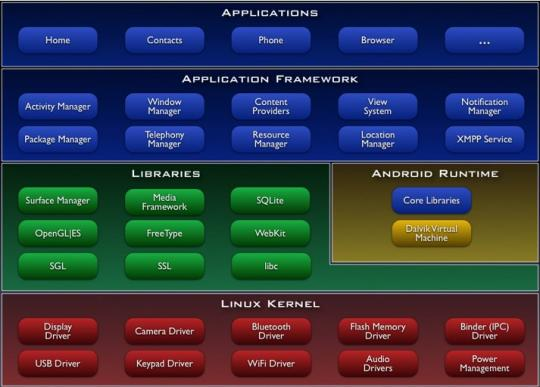
\includegraphics[width = 90mm]{images/androidSystemArchitecture.jpg}
				\caption[Android System Architecture]{[3] Android System Architecture}
			\end{figure}
			
		\subsection{Applications, Activities and Services}
			
			\subsubsection{Applications}
				Android apps are written in the Java programming language. The Android SDK tools compiles the code, along with any data and resource files into an APK (Android Package), which is an archive file with an .apk suffix. One APK file contains all the contents of an Android app and is the file that Android-powered devices use to install the app [6]. The Android operating system is a multi-user Linux system in which each app is a different user. Each process has its own virtual machine (VM), so an app's code runs in isolation from other apps. By default, every app runs in its own Linux process.
				
			\subsubsection{Activities}
				An Activity is an application component that provides a screen with which users can interact in order to do something, such as dial the phone, take a photo, send an email, or view a map [7]. An application usually consists of multiple activities that are loosely bound to each other. Typically, one activity in an application is specified as the main activity, which is presented to the user when launching the application for the first time. Each activity can then start another activity in order to perform different actions.
				
			\subsection{Services}
				A Service is an application component that can perform long-running operations in the background and does not provide a user interface [8]. Another application component can start a service and it will continue to run in the background even if the user switches to another application. Additionally, a component can bind to a service to interact with it and even perform IPC (Inter Process Communication). For example, a service might handle network transactions, play music, perform file I/O, or interact with a content provider, all from the background.
					 	
	\section{Growth of available RAM over the years}
		
		\subsection{Advances in Technology}
			RAM is a form of computer data storage. A RAM device allows data items to be accessed (read or written) in almost the same amount of time irrespective of the physical location of data inside the memory. The overall goal of using a RAM device is to obtain the highest possible average access performance while minimizing the total cost of the entire memory system. Today, random-access memory takes the form of IC (Integrated Circuits)(s).
		
			\subsubsection{Moore's Law}
				Moore's law is the observation that the number of transistors in a dense IC doubles approximately every two years.
				
				\begin{figure}[h]
					\centering
					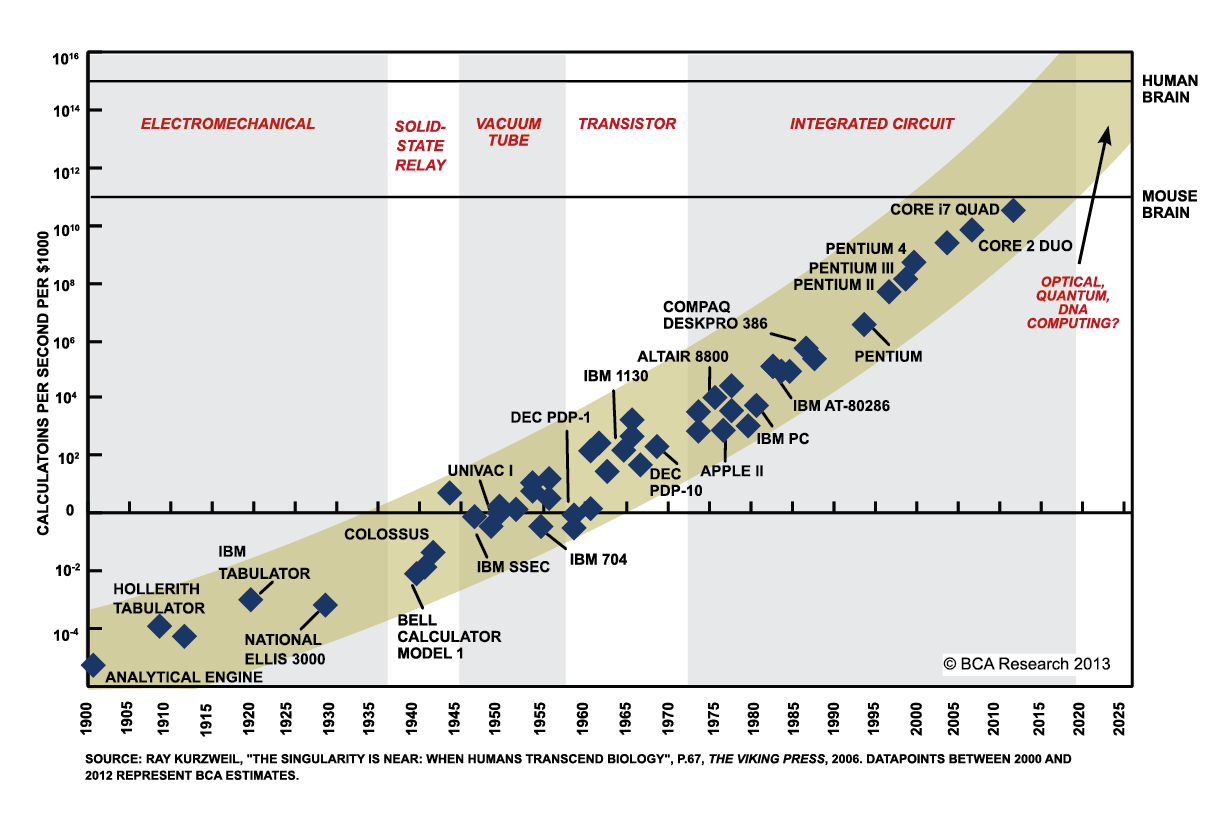
\includegraphics[width = 90mm]{images/mooresLaw.png}
					\caption[Moore's law]{[9] Moore's Law}
				\end{figure}
				
				Advancements in digital electronics are strongly linked to Moore's law, especially in the context of memory capacity. T-Mobile G1, the very first Android smart-phone to be released back in 2008 [10] has a 256 MB (Mega-Byte) RAM [11]. In comparison, the Nexus 6P that was released in September 2015 has a 3 GB (Giga-Byte) RAM and some devices like the LG T585 have a 16 GB RAM [12][13], which amounts to 64 times the memory capacity of the T-Mobile G1. The rapid growth in the amount of RAM available to Android devices has in part led to newer possibilities and in our case, a better CRA for determining which processes (in the context of Android applications) remain in memory.
			 	
		\subsection{Demise of Task Killers}
			One of the main benefits of the Android OS is the fact that unlike certain other OS(s), it can run apps in the background. This enables us to have multiple applications open at the same time which results in true multitasking. Thus, RAM availability is highly desirable [14]. A popular misconception is that forcibly removing applications from memory in order to 'free up RAM' will result in increased performance. In fact, several task-killer applications promise to do precisely that. With the advancement in the amount of RAM available, the debate should be about how to better use all this extra space, not killing applications to 'free up' more space. In fact, the Android OS can go one step further and pro-actively cache applications that the user might use in the near future. We'll analyze this prospect in more detail in the upcoming chapters.  
			
	\section{How Android Manages Processes}
		
		\subsection{Android Process Lifecycle}
			A Android process can be in one of five different states at any given time, from most important to least important [15]:
			
			\begin{itemize}
				\item Foreground process: A foreground process is one that is required for what the user is currently doing.
				
				\item Visible process: A visible process is one holding an Activity that is visible to the user on-screen but not in the foreground.
				
				\item Service Process: Service processes are not directly visible to the user, they are generally doing things that the user cares about (such as playing music in the background). 
				
				\item Background process: A background process is one holding an Activity that is not currently visible to the user. They are kept in an LRU list to ensure the process that was most recently seen by the user is the last to be killed when running low on memory.  
				
				\item Empty process: An empty process is one that doesn't hold any active application components. The only reason to keep such a process around is as a cache to improve startup time the next time a component of its application needs to run.				
			\end{itemize}
			
			Every Android smart-phone user is capable of checking the processes that currently reside in physical memory. The Application Manager which is part of the Settings app shows a list of running processes and cached background processes. Additionally, it breaks down the composition of RAM usage by the System applications and user installed applications. 
			
			\begin{figure}[h]
				\centering
				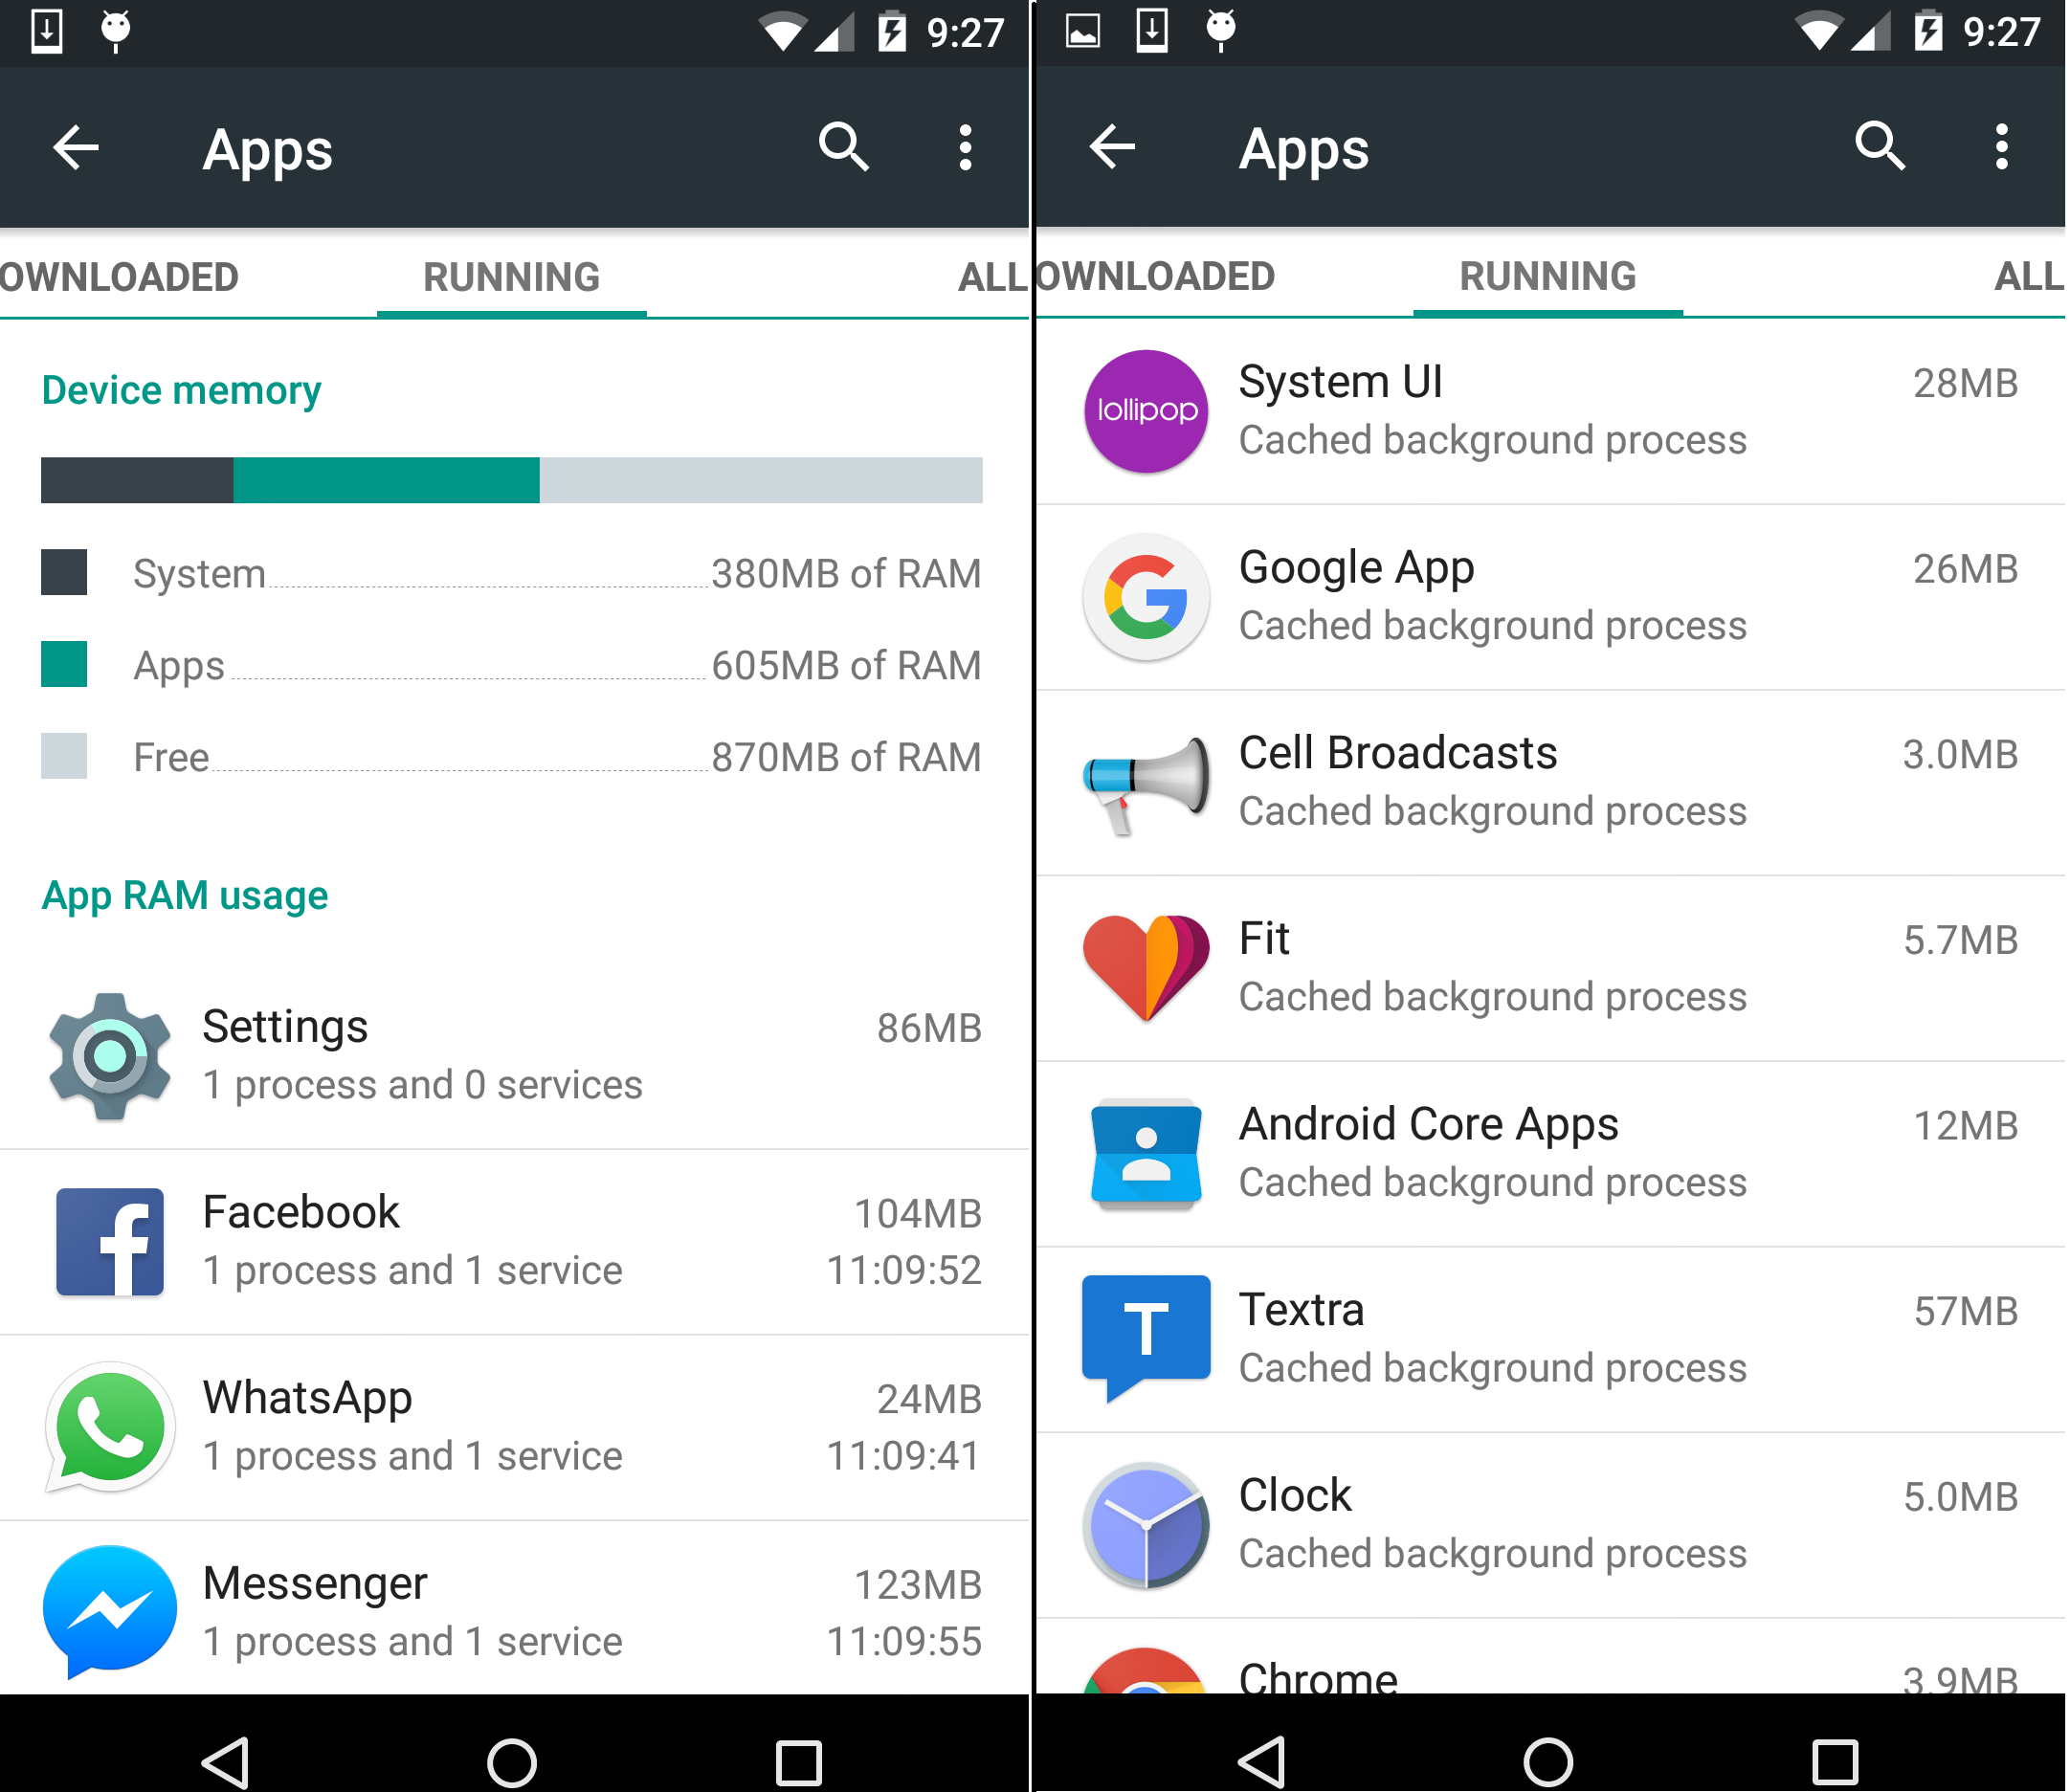
\includegraphics[width = 90mm]{images/runningApps.png}
				\caption[Running Apps and Cached Background Processes]
				{Left - List of Running Applications (Active Processes and Services)\\
					Right - List of Cached Background Processes}
			\end{figure}			
			 
		\subsection{LRU Cache}
			LRU is a CRA that discards the least recently used items first. This algorithm requires keeping track of what was used when, which is expensive if one wants to make sure the algorithm always discards the least recently used item [17]. Android keeps processes that are not hosting a foreground app component in a LRU cache. As the system runs low on memory, it may kill processes in the LRU cache beginning with the process least recently used, but also giving some consideration toward which processes are most memory intensive [16].
			
	\section{Goals and Objectives}
		
		\subsection{A User-Centric CRA}
			The main benefit of caching processes (components of applications recently clicked by the user) in memory is to improve startup time (of the application), the next time a component of the application needs to run. This greatly enhances the usability experience and therefore it's in Android's best interests to increase the efficiency of this cache i.e. improve its CHR. In addition to recency of application usage (which is what Android currently relies on in the form of LRU as a CRA), there is scope to potentially infer what application a user may click in the near future. A more user-centric CRA could look into contextual clues and deduce patterns in user behavior to improve the decision making involved in determining which applications to cache in memory, pro-actively or otherwise. We will explore in theoretical detail many such possibilities for user behavior inference and as a proof of concept, read the user's Calendar  application and parse for contextual information that could help in improving the CHR of the APC (Android Process Cache). 

	\section{Organization of Thesis}
		Several works in the past have focused on context-aware applications and ways to observe user behavior patterns. We'll explore some these works and how this contextual data was put to use in Section 2. In Section 3, we'll take a look at some of the challenges in collecting cache metrics like detecting what's in the RAM, detecting when the user clicks a new application, whether to approach the problem at the user level or the system level, to list a few. Section 4 elaborates on the setup of the experiment and analyzes the design of the applications used to collect these metrics. We dive into the data in Section 5 and summarize its ramifications. We also investigate how certain factors could explain the variation in data. Section 6 talks about scope for future work and explores some of the possibilities of directly adding to this work. We conclude the thesis with Section 7.  


%				How to Refer to a table, look below:

%[ Insert your text to chapter 1 here.  A pretend example of a silly
%table is provided below (i.e., Table~\ref{SILLY}).~]

%								Table Template


%     \vfill
%     \begin{table}[ht]
%     \caption{A silly glossary for research reports.\label{SILLY}}
%     \begin{center}
%     \begin{tabular}{p{2.75in}|p{2.5in}}
%      \rule[-0.5em]{0pt}{1.75em} \bf When Professors write \ldots
%      & \bf they REALLY mean \ldots \\ \hline\hline
%      %--------+------------------------------------
%      \rule[-0.5em]{0pt}{1.75em} Typical results are shown \ldots
%      & The best results are shown \ldots \\ \hline
%      %--------+------------------------------------
%      \rule[-0.5em]{0pt}{1.75em} It is generally believed that
%      \ldots & A couple of other guys think so too  \\ \hline
%      %--------+------------------------------------
%      \rule[-0.5em]{0pt}{1.75em}Thanks to Al K.~Seltzer for
%      assistance and to I.P. Daly for valuable discussions &
%      Seltzer did the work and Daly explained
%      what it meant \\
%     \end{tabular}
%     \end{center}
%     \end{table}
%     \vfill

%XXXXXXXXXXXXXXXXXXXXXXXXXXXXXXXXXXXXXXXXXXXXXXXXXXXXXXXXXXXXXXXXXXXX
%XXXXXXXXXXXXXXXXXXXXXXXXXXXXXXXXXXXXXXXXXXXXXXXXXXXXXXXXXXXXXXXXXXXX
%XXXXXXXXXXXXXXXXXXXXXXXXXXXXXXXXXXXXXXXXXXXXXXXXXXXXXXXXXXXXXXXXXXXX
%XXXXXXXXXXXXXXXXXXXXXXXXXXXXXXXXXXXXXXXXXXXXXXXXXXXXXXXXXXXXXXXXXXXX

\chapter{Related Work}
	
	\section{Early Studies in Context-Aware Computing}
		Dey, Abowd and Salber, in their 2001 paper titled {\em A conceptual framework and a toolkit for supporting the rapid prototyping of context-aware applications} laid out the foundation and in many ways a standardized framework for building context-aware applications. When this paper was published, mobile phones were becoming mainstream devices and were no longer confined to the hands of the wealthy. By definition, more people were mobile and the devices they carried with them had the potential to utilize contextual information gathered from the surroundings, in ways that desktops could'nt do due to their stationary nature. They defined context as any information that characterizes a situation related to the interaction between humans, applications and the surrounding environment. They opined that the state of research in context-awareness was inadequate for three main reasons:
		
		\begin{itemize}
			\item The notion of context was ill-defined.
			\item There was a lack of conceptual models and methods to help drive the design of context-aware applications.
			\item No tools were available to jump-start the development of context-aware applications.
		\end{itemize}
		
		 They focused their efforts on the pieces of context that could be inferred automatically from sensors in a physical environment and produced Context Toolkit [20], a conceptual framework that supported the rapid development of context-aware applications. It is important to keep in mind that at the time this paper was published, the notion of what we refer to as a smart-phone was non-existent. This is evident from the fact that most APMD(s) have built-in sensors that measure motion, orientation, and various environmental conditions. These sensors are capable of providing raw data with high precision and accuracy, and are useful in monitoring three-dimensional device movement or positioning, or changes in the ambient environment near a device [21]. These conditions make APMD(s) very suitable for utilizing contextual information and translating that potential into a better user experience. We utilize this feature of APMD(s) to propose ways to improve user experience by incorporating contextual information in managing the physical memory of the APMD.		
			
	\section{Context Patterns in Application Usage}
		Several works have attempted to collect user behavior data and they've accomplished this in unique ways. Hannu Verkasalo, in his 2007 paper titled {\em Contextual Patterns in Mobile Service Usage} analyzes how mobile services are used in different contexts [18]. Usage contexts were divided into {\em home, office} and {\em on the move}. A specialized algorithm tracked user's location patterns over a period of time to determine whether the user was at home or at work. Furthermore, changes in location data revealed whether the user was in transit between home and work. There was a correlation between the mobile services requested by the user and the user's physical location, which enabled the algorithm to understand the user's context quite well (refer Figure 2-1). It was also observed that certain services were requested more during the weekends as opposed to certain others being requested more during the weekdays i.e. days with office hours.  
		
		\begin{figure}[!ht]
			\centering
			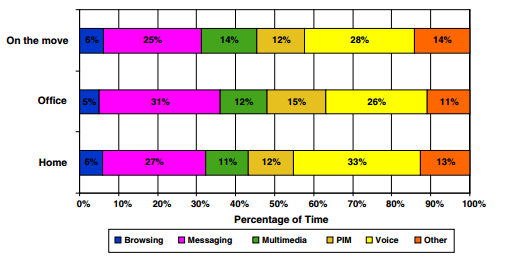
\includegraphics[width = 90mm]{images/appsByTime.png}
			\caption[Mobile Services Requested At Various Times Of Day]
			{By classifying user context into three distinct entities namely {\em home, work} and {\em on the move}, the author managed to infer which services were requested more in a given context. For e.g. Voice services i.e. calling was predominantly requested while the user was at home. This type of information can be very useful.}
		\end{figure}
	
	\section{Context Phone}
		Mika Raento, Antti Oulasvirta, Renaud Petit, and Hannu Toivonen, in their paper titled {\em ContextPhone: A Prototyping Platform for Context-Aware Mobile Applications} proposed that mobile phones are well suited for context aware computing due to an intimate relationship between the user and the phone [19]. Their primary goal was to provide context as a resource and in order to accomplish that, developed a {\em ContextPhone} which comprised of four components (Refer Figure 2-2):
		
		\begin{itemize}
			\item Sensors that acquire contextual data (such as location data from GPS)
			\item Communication services (such as SMS, MMS to list a few)
			\item Customizable Applications (that can replace existing applications)
			\item System Services (such as background services for error logging)
		\end{itemize}
		
		
		\begin{figure}[!ht]
			\centering
			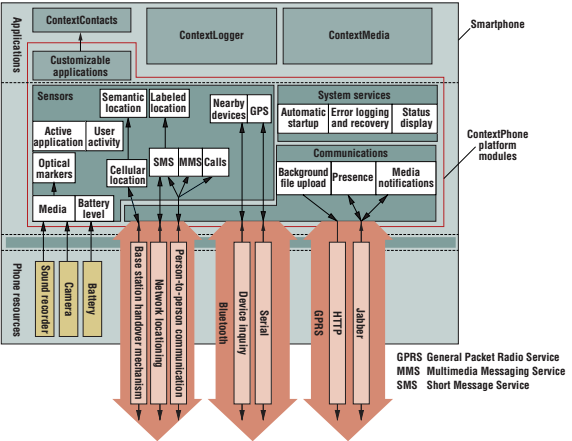
\includegraphics[width = 90mm]{images/contextPhone.png}
			\caption[Context Phone]
			{The ContextPhone platform; Four interconnected components — sensors, system services, communication services, and customizable applications — facilitate communication with the outside world.}
		\end{figure}
		
		It is important to observe that this paper came out in 2005, two years before the first version of Android was even launched. Yet, their fundamental point of focus is still relevant in how we can use context as a powerful resource. Their point about the necessity of customizable applications that are needed for context information to be relevant perfectly applies to this thesis. The Android OS which is open sourced as AOSP is as customizable as it can get when it comes to modifying mobile components and by extension the user experience with APMD(Android Powered Mobile Device)(s). To be specific, it facilitates ways to gather cache related information such as the list of processes currently residing in memory, the current foreground application and whether the caching mechanism per se is up for modification to list a few. It would be impossible to collect and/or modify such information on any other mobile OS (such as Apple's iOS).
		
	\section{Using Context Information for Authentication}
		Dey et al. established a framework for collecting contextual data and Verkasalo and Raento et al. have shown how user behavior can be analyzed through sensors and other modules that gather contextual information. Shi et al.'s paper titled {\em Implicit Authentication through Learning User Behavior} demonstrates a similar approach in collecting behavioral data of the user but differ in how they put that information to use. They have devised a model to implicitly authenticate smart-phone users based on their behavioral patterns. The user's usage patterns are collected (for e.g. how many calls a user makes a day, how many times user's location changes (Refer Figure 2-3) etc.) and this information is used in building a user model [22].  
		
		\begin{figure}[!ht]
			\centering
			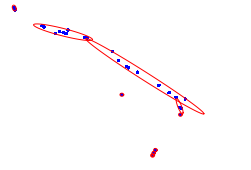
\includegraphics[width = 90mm]{images/gpsTrace.png}
			\caption[User's GPS Trace]
			{The blue dots represent the user’s traces in a two-hour epoch over multiple days, and the red ellipses represent the clusters fitted. The major two directional clusters correspond to the user’s trajectory on a highway}
		\end{figure}		
		Once the user model is built and the profile completed, the algorithm can determine the likelihood of a random user of the phone not being the owner of the phone (the one whose user model was profiled). 
		
		As demonstrated by Shi et al., there are numerous ways contextual information can come in handy. In our case, we propose a user-centric CRA for the APC, demonstrate its superior efficiency and user experience, by looking into the user's calendar for contextual information.  			
	
\chapter{Challenges in Collecting the Desired Metrics}
	
	\section{Introduction}
		Now that we've laid the foundation for using contextual information to influence which processes Android caches in memory, we need to establish the metrics that need to be collected in order to measure the efficiency of the existing CRA and the proposed CRA. The following section addresses the metrics we need.
	
	\section{What are the desired metrics?}
		
		\subsection{Hits, Misses, Hit Ratio \& Latency}
			Alan Jay Smith defines Cache as a high speed buffer that holds items in current use [23]. In our context, Android holds application components (such as processes) as CBP (Cached Background Process)(s) in memory. As previously discussed, CBP(s) do not take up processor time, they are merely cached for quick application startup should the user request that particular application. A cache hit is a state in which data requested for processing by a component or application is found in the cache memory. It is a faster means of delivering data to the processor, as the cache already contains the requested data [24]. When applied to our scenario, a cache hit would represent a situation wherein the user requests (clicks) an application that currently resides in memory, either as an active process (including services) or as a CBP (Refer Figure 3-1).  
			
			\begin{figure}[!ht]
				\centering
				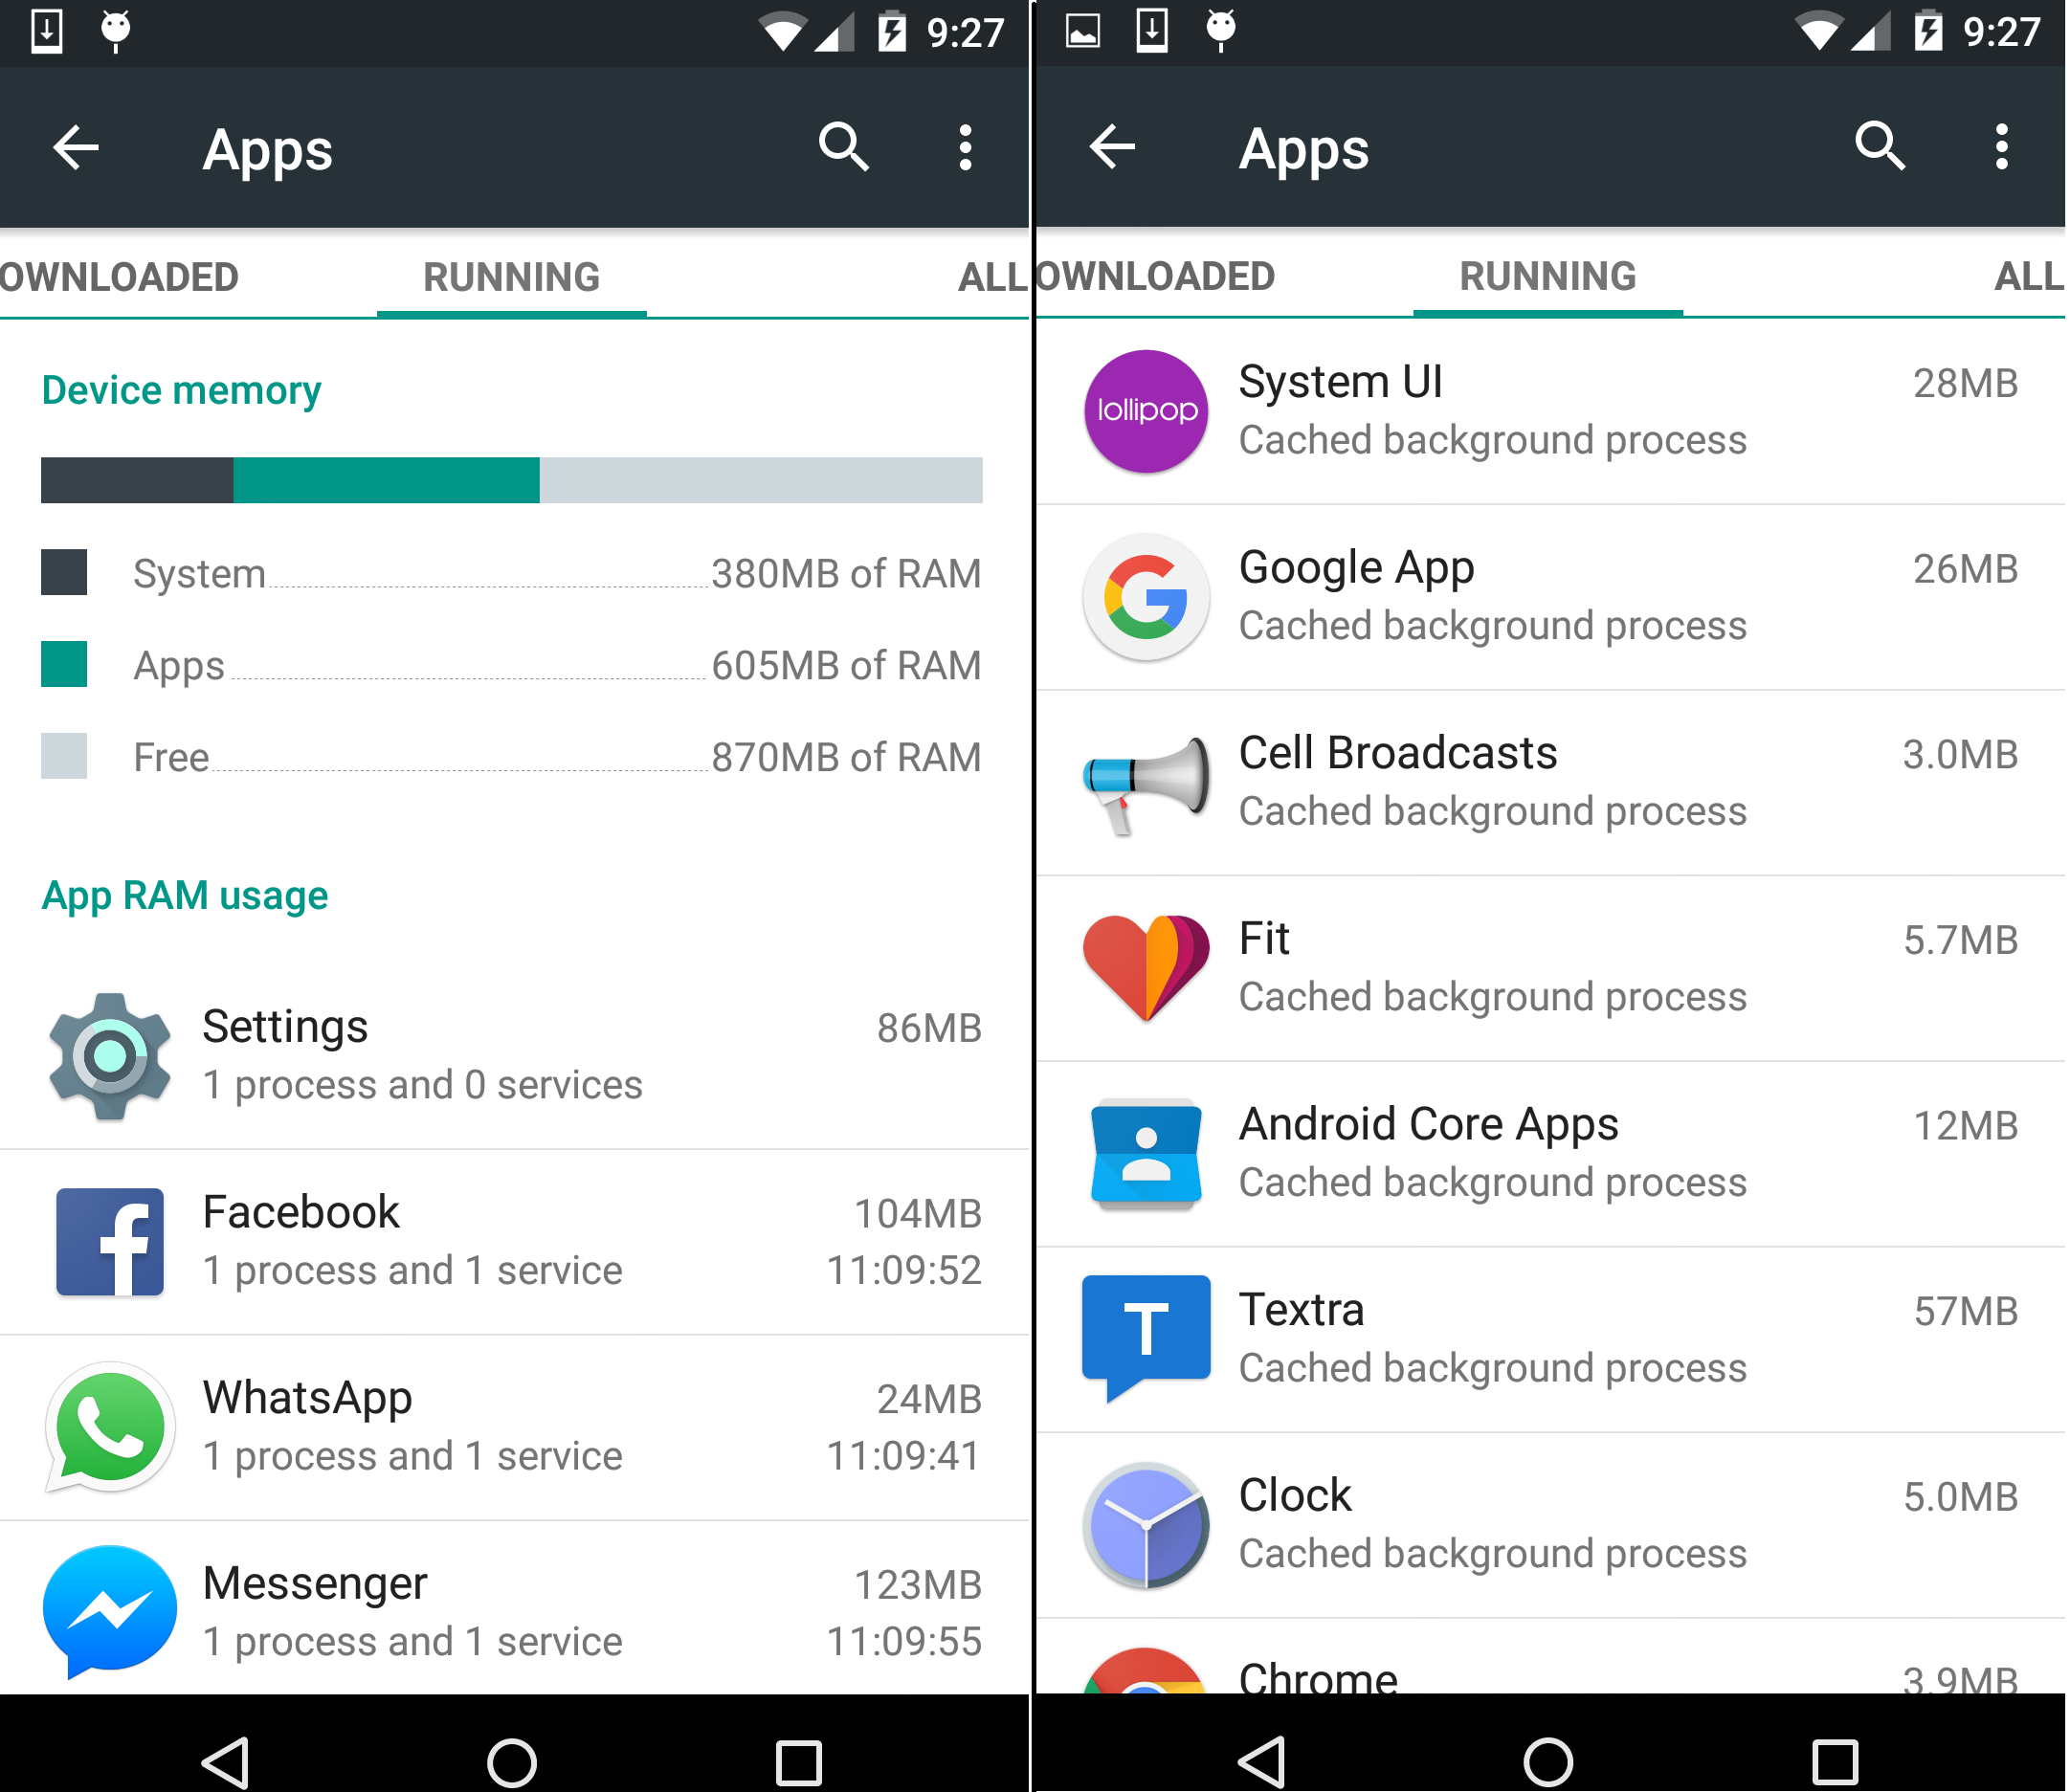
\includegraphics[width = 90mm]{images/runningApps.png}
				\caption[Running Apps and CBP(s) - Cache Hit]
				{Given this snapshot of the RAM, if the user clicks on the Messenger application (active process) or Clock application (CBP), it would result in a Cache Hit}
			\end{figure}
			
			A cache miss is a state where the data requested for processing, by a component or application is not found in the cache memory [25]. When applied to our scenario, a cache miss would represent a situation wherein the user requests (clicks) an application that currently does not reside in memory, either as an active process (including services) or as a CBP (Refer Figure 3-2).
			
			\begin{figure}[!ht]
				\centering
				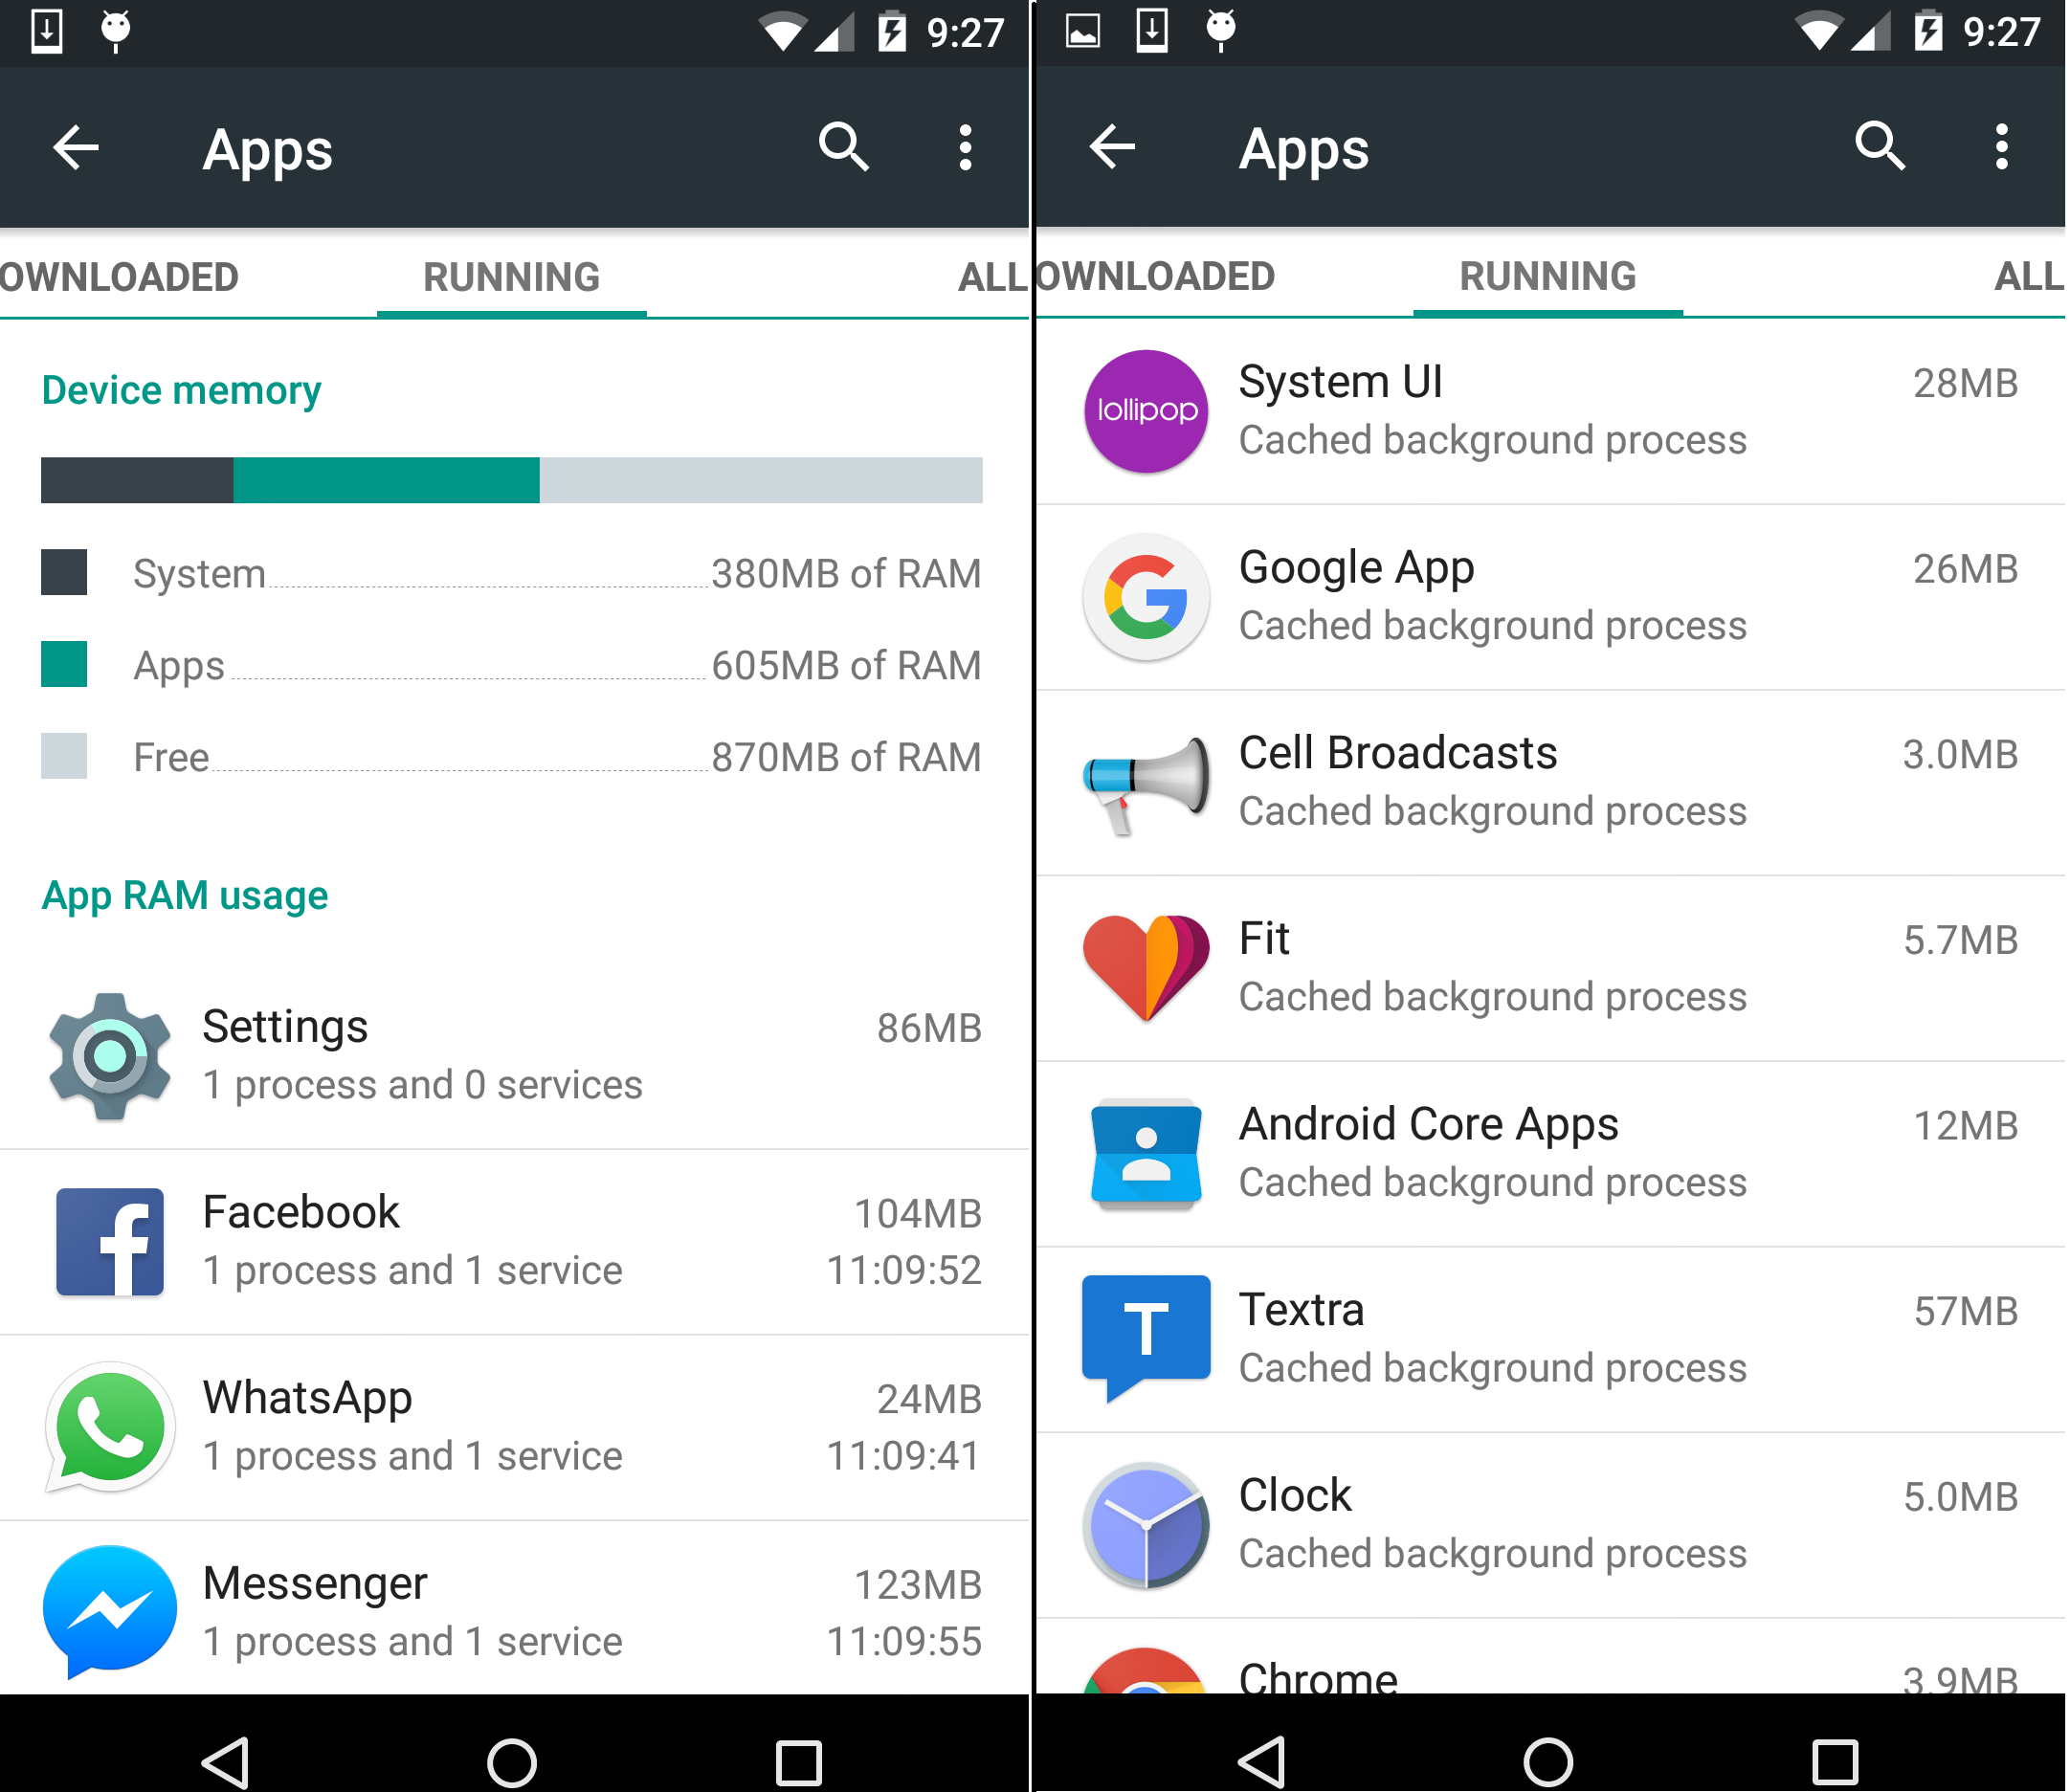
\includegraphics[width = 90mm]{images/runningApps.png}
				\caption[Running Apps and CBP(s) - Cache Miss]
				{Given this snapshot of the RAM, if the user clicks on say, the Google Drive application (process not in memory), it would result in a Cache Miss}
			\end{figure}		
			
			CHR is defined as the percentage of cache hits compared to the overall number of requests (total of cache hits and cache misses).
			
			\begin{eqnarray}
				Overall Number Of Requests = Cache Hits + Cache Misses \label{Total Requests} \\
				CHR = \frac{Cache Hits}{Overall Number Of Requests} * 100 \label{CHR}
			\end{eqnarray}
			
			There are two primary figures of merit of a cache [23]:
			
			\begin{itemize}
				\item Latency
				\item CHR
			\end{itemize}
			
			The latency of a cache describes how long after requesting a desired item, the cache can return that item (in the case of a cache hit). In our scenario, processes are cached in RAM. Therefore, even if the number of processes cached in memory increases, there will hardly be any difference in the time it takes to fetch a reque-sted item (application component) as they all reside in RAM which by definition supports random access. Latency is more of a factor in caches that are located further away from physical memory (such as L1 and L2 caches).
			
			The CHR of a cache describes how often a searched-for item is actually found in the cache. The higher the CHR, the better the cache is. When applied to our context, a high CHR results is more application components being fetched from memory, rather than disk which in turn results in quicker application startup times. This improvent in startup speed results in an enhanced user experience.   
		
		\subsection{CRA(s) Under Consideration}
			Now that we've determined the fundamental metrics we need, let's analyze the various CRA(s) including the one Android currently uses, namely LRU.
			
			\subsubsection{Optimal CRA}
				The most efficient CRA would be to always discard the information that will not be needed for the longest time in the future. In our case, the ideal CRA would be one that ensures that every application the user requests, resides in memory. This optimal result is referred to as Belady's optimal algorithm [26] or the clairvoyant algorithm. Since it is generally impossible to predict how far in the future information will be needed, this is not implementable in practice. The practical minimum can be calculated only after experimentation, and one can compare the effectiveness of the actually chosen CRA against Belady's as a benchmark.
			
			\subsubsection{LRU}
				This is the default CRA Android currently uses to discard processes from memory. LRU is a type of CRA that discards the least recently used items first. This algorithm keeps track of what was used when, and it's expensive to ensure that the least recently used item is always discarded first. When applied to our scenario, Android caches application components in memory as CBP(s) and associates each with a timestamp. If the memory gets too full, it starts removing the least frequently used CBP(s) first and depending on how direly low the memory is, it may not stop killing processes until even the active foreground application (the one user is interacting with) is removed, [15] although this situation is extremely rare in practice and only results in the case of malfunctioning applications that leak memory. The Settings application can give the user clues about which CBP(s) were recently used. Clicking on an application that is currently not in memory results in that application being cached as a CBP near the top of the list. This suggests that the CBP(s) displayed by the Settings application are roughly sorted by their timestamp from MRU to LRU (Refer Figure 3-3). 
				
				\begin{figure}[!ht]
					\centering
					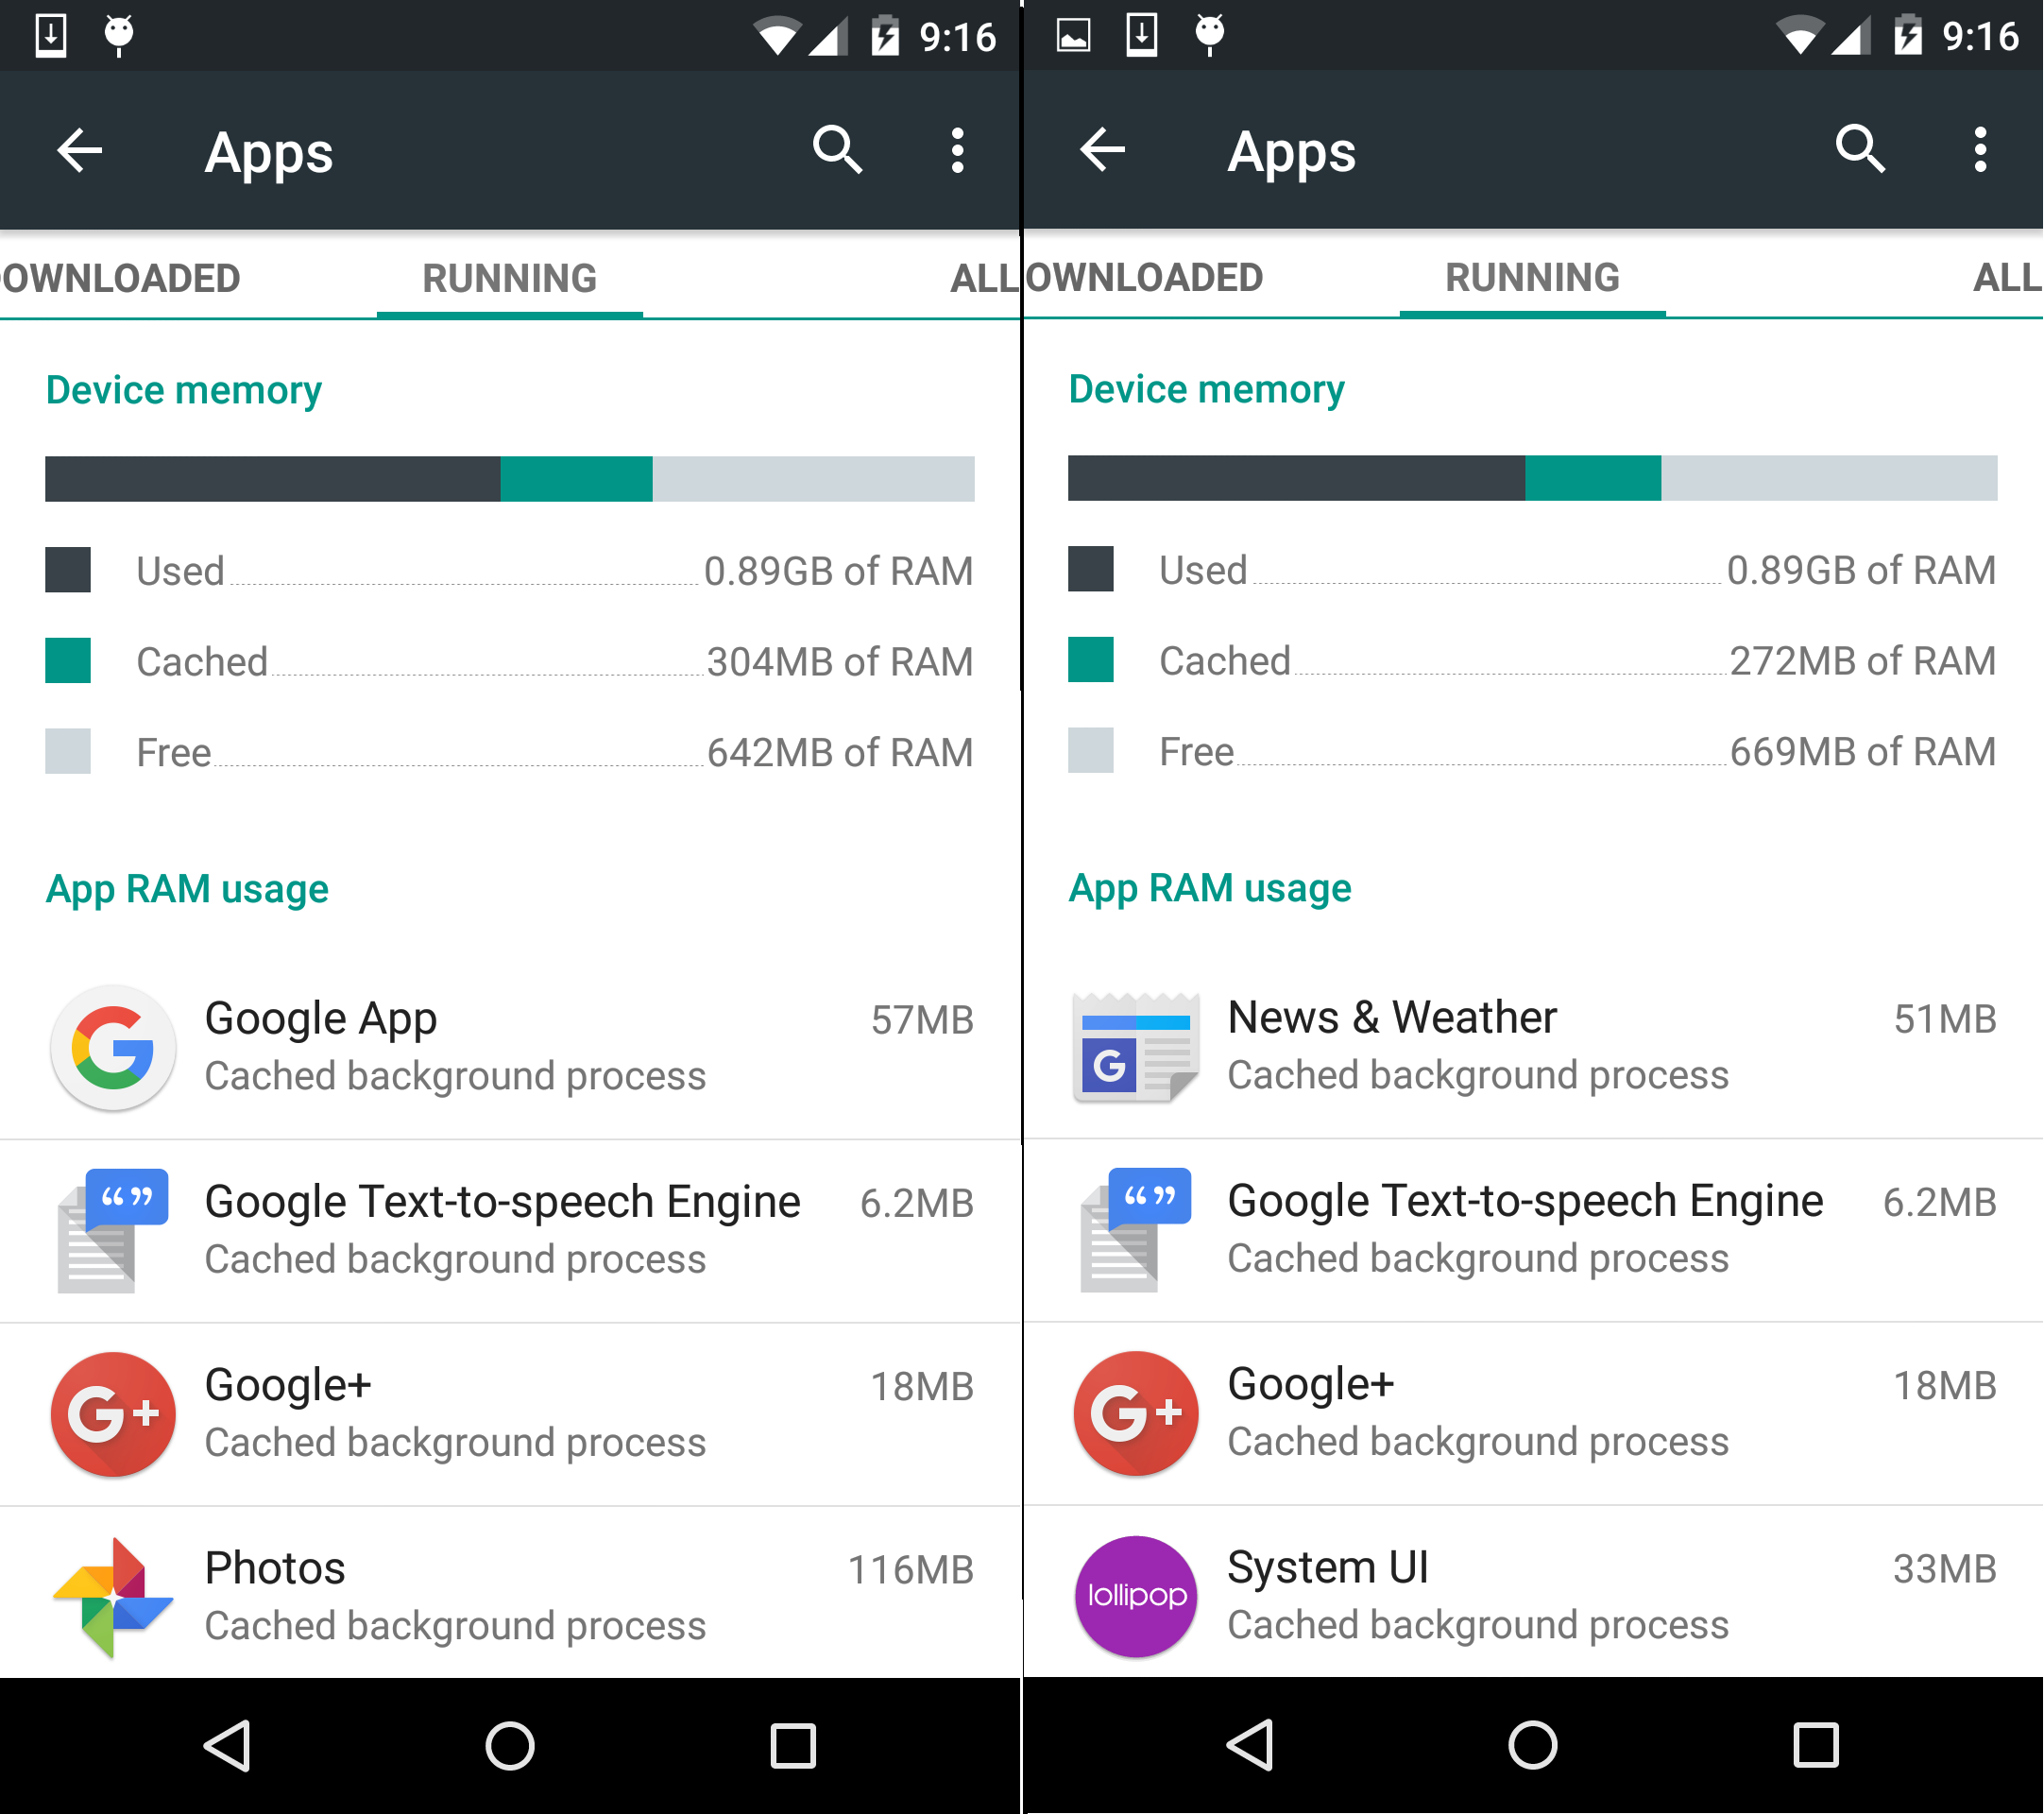
\includegraphics[width = 90mm]{images/beforeAndAfterNews.png}
					\caption[Before \& After News App Launch]
					{The image to the left describes the snapshot of the CBP(s) as displayed to the end-user by the Settings app. The image to the right displays the snapshot of the CBP(s) after the end-user requests for the News and Weather application. Note that the News and Weather application will not be cached as a CBP until the user is done interacting with it as up until that point, it will reside in memory as an active process.}
				\end{figure}				
				
				It is worth noting that a perfect implementation of LRU requires a timestamp on each reference, and the OS needs to keep a list of items ordered by the timestamp. This implementation may be deemed too expensive in certain cases especially if the frequency of memory references is high. The common practice is to approximate the LRU behavior and this can be achieved in other ways [27].
				 
			\subsubsection{Most Recently Used (MRU)}
				MRU discards, in contrast to LRU, the most recently used items first. In findings presented at the 11th VLDB conference, Chou and DeWitt noted that when a file is being repeatedly scanned in a looping sequential reference pattern, MRU was the best replacement algorithm [28]. Subsequently other researchers presenting at the 22nd VLDB conference noted that for random access patterns and repeated scans over large datasets (sometimes known as cyclic access patterns) MRU cache algorithms had more hits than LRU due to their tendency to retain older data [29]. In our scenario, CBP(s) neither comprise a 'large dataset' nor are they repeatedly scanned in a looping sequential reference pattern (as they are only invoked during application requests which are on average, not that often), therefore it's unlikely that MRU would result in a high CHR but it's worth mentioning nonetheless. MRU algorithms are most useful in situations where the older an item is, the more likely it is to be accessed, which again is not a feature of CBP(s).			
			
			\subsubsection{Least Frequently Used (LFU)}
				LFU is a type of CRA usually associated with memory management within a computer. The standard characteristics of this method involve the system keeping track of the number of times an item is referenced in memory. When the cache is full and requires more room the system will purge the item with the lowest reference frequency. This could be a really good fit with our scenario given the tendency of most smart-phone users to stick with the same set of popular applications and use them in rotation [31]. Under these circumstances, the frequency of a select few applications would be really high and would always be cached in memory as they're requested often. LFU is sometimes combined with a Least Recently Used algorithm called LRFU [30]. We'll explore some of the possibilities with LFU in the future scope section and in our proposed hybrid approach where we incorporate global frequency of application usage in obtaining contextual information.
				 
			\subsubsection{Random Replacement (RR)}
				Much like the name suggests RR is a CRA that randomly selects a candidate item and discards it to make space when necessary. This algorithm does not require keeping any information about the access history. For its simplicity, it has been used in ARM processors [32]. When applied to our scenario, it does'nt seem like a viable option, mainly because there is'nt a benefit in randomly caching applications in memory.
				 
			\subsubsection{LRU - Context Hybrid}
				So far we've analyzed the standard CRA(s) that focus on discarding items that were either accessed least recently, least frequently or in other standard ways. Our approach combines the applications that Android caches through an LRU scheme with a separate context-analyzer module that reads the user's calendar and predicts which applications the user is likely to use. When the user requests an application, the combined set of applications (default applications in LRU and the list of suggested applications) is used as the base to predict whether a cache hit or cache miss occurred. We'll analyze in detail how each module functions but before that, let's take a look at whether Android caches CBP(s) pro-actively and how applications will be removed from memory in the cases where it runs too low.
				
				\paragraph{Pro-actively Adding CBP(s)}
					In order for the proposed LRU-Context Hybrid (henceforth referred to as the Hybrid approach) CRA to work, there must be provision for the Android OS to pro-actively cache application components in memory as CBP(s). Presuming that the context-analyzer module does its job and suggests a list of applications the user might use in the near future (based on user's Calendar information), there must a mechanism for Android to utilize that information and pro-actively cache these applications in RAM as CBP(s). This mechanism can be verified at the user level through a small experiment. As previously mentioned, the Settings application provides a visual interface for the list of active processes and services running in memory and the CBP(s) that reside in memory at any moment in time. As part of the experiment, each and every CBP was forcefully removed from the cache (there is provision to do this at the user level (Refer Figure 3-4)). 
						
					\begin{figure}[!ht]
						\centering
						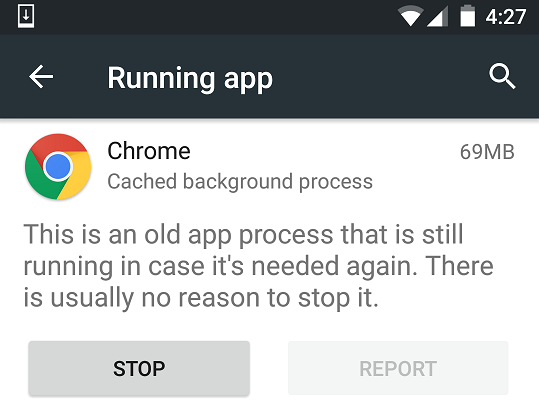
\includegraphics[width = 90mm]{images/removeCBP3.png}
						\caption[Remove CBP]
						{Pressing the {\em STOP} button removes the CBP from memory}
					\end{figure}					
					
					Once each CBP was removed, the phone was untouched for three minutes. After three minutes, when the Settings application was launched to look at the list of CBP(s), it wasn't empty. Instead, there were several CBP(s), some of which were previously removed and some of which were'nt in the list to begin with (Refer Figure 3-5). 
					
					\begin{figure}[!ht]
						\centering
						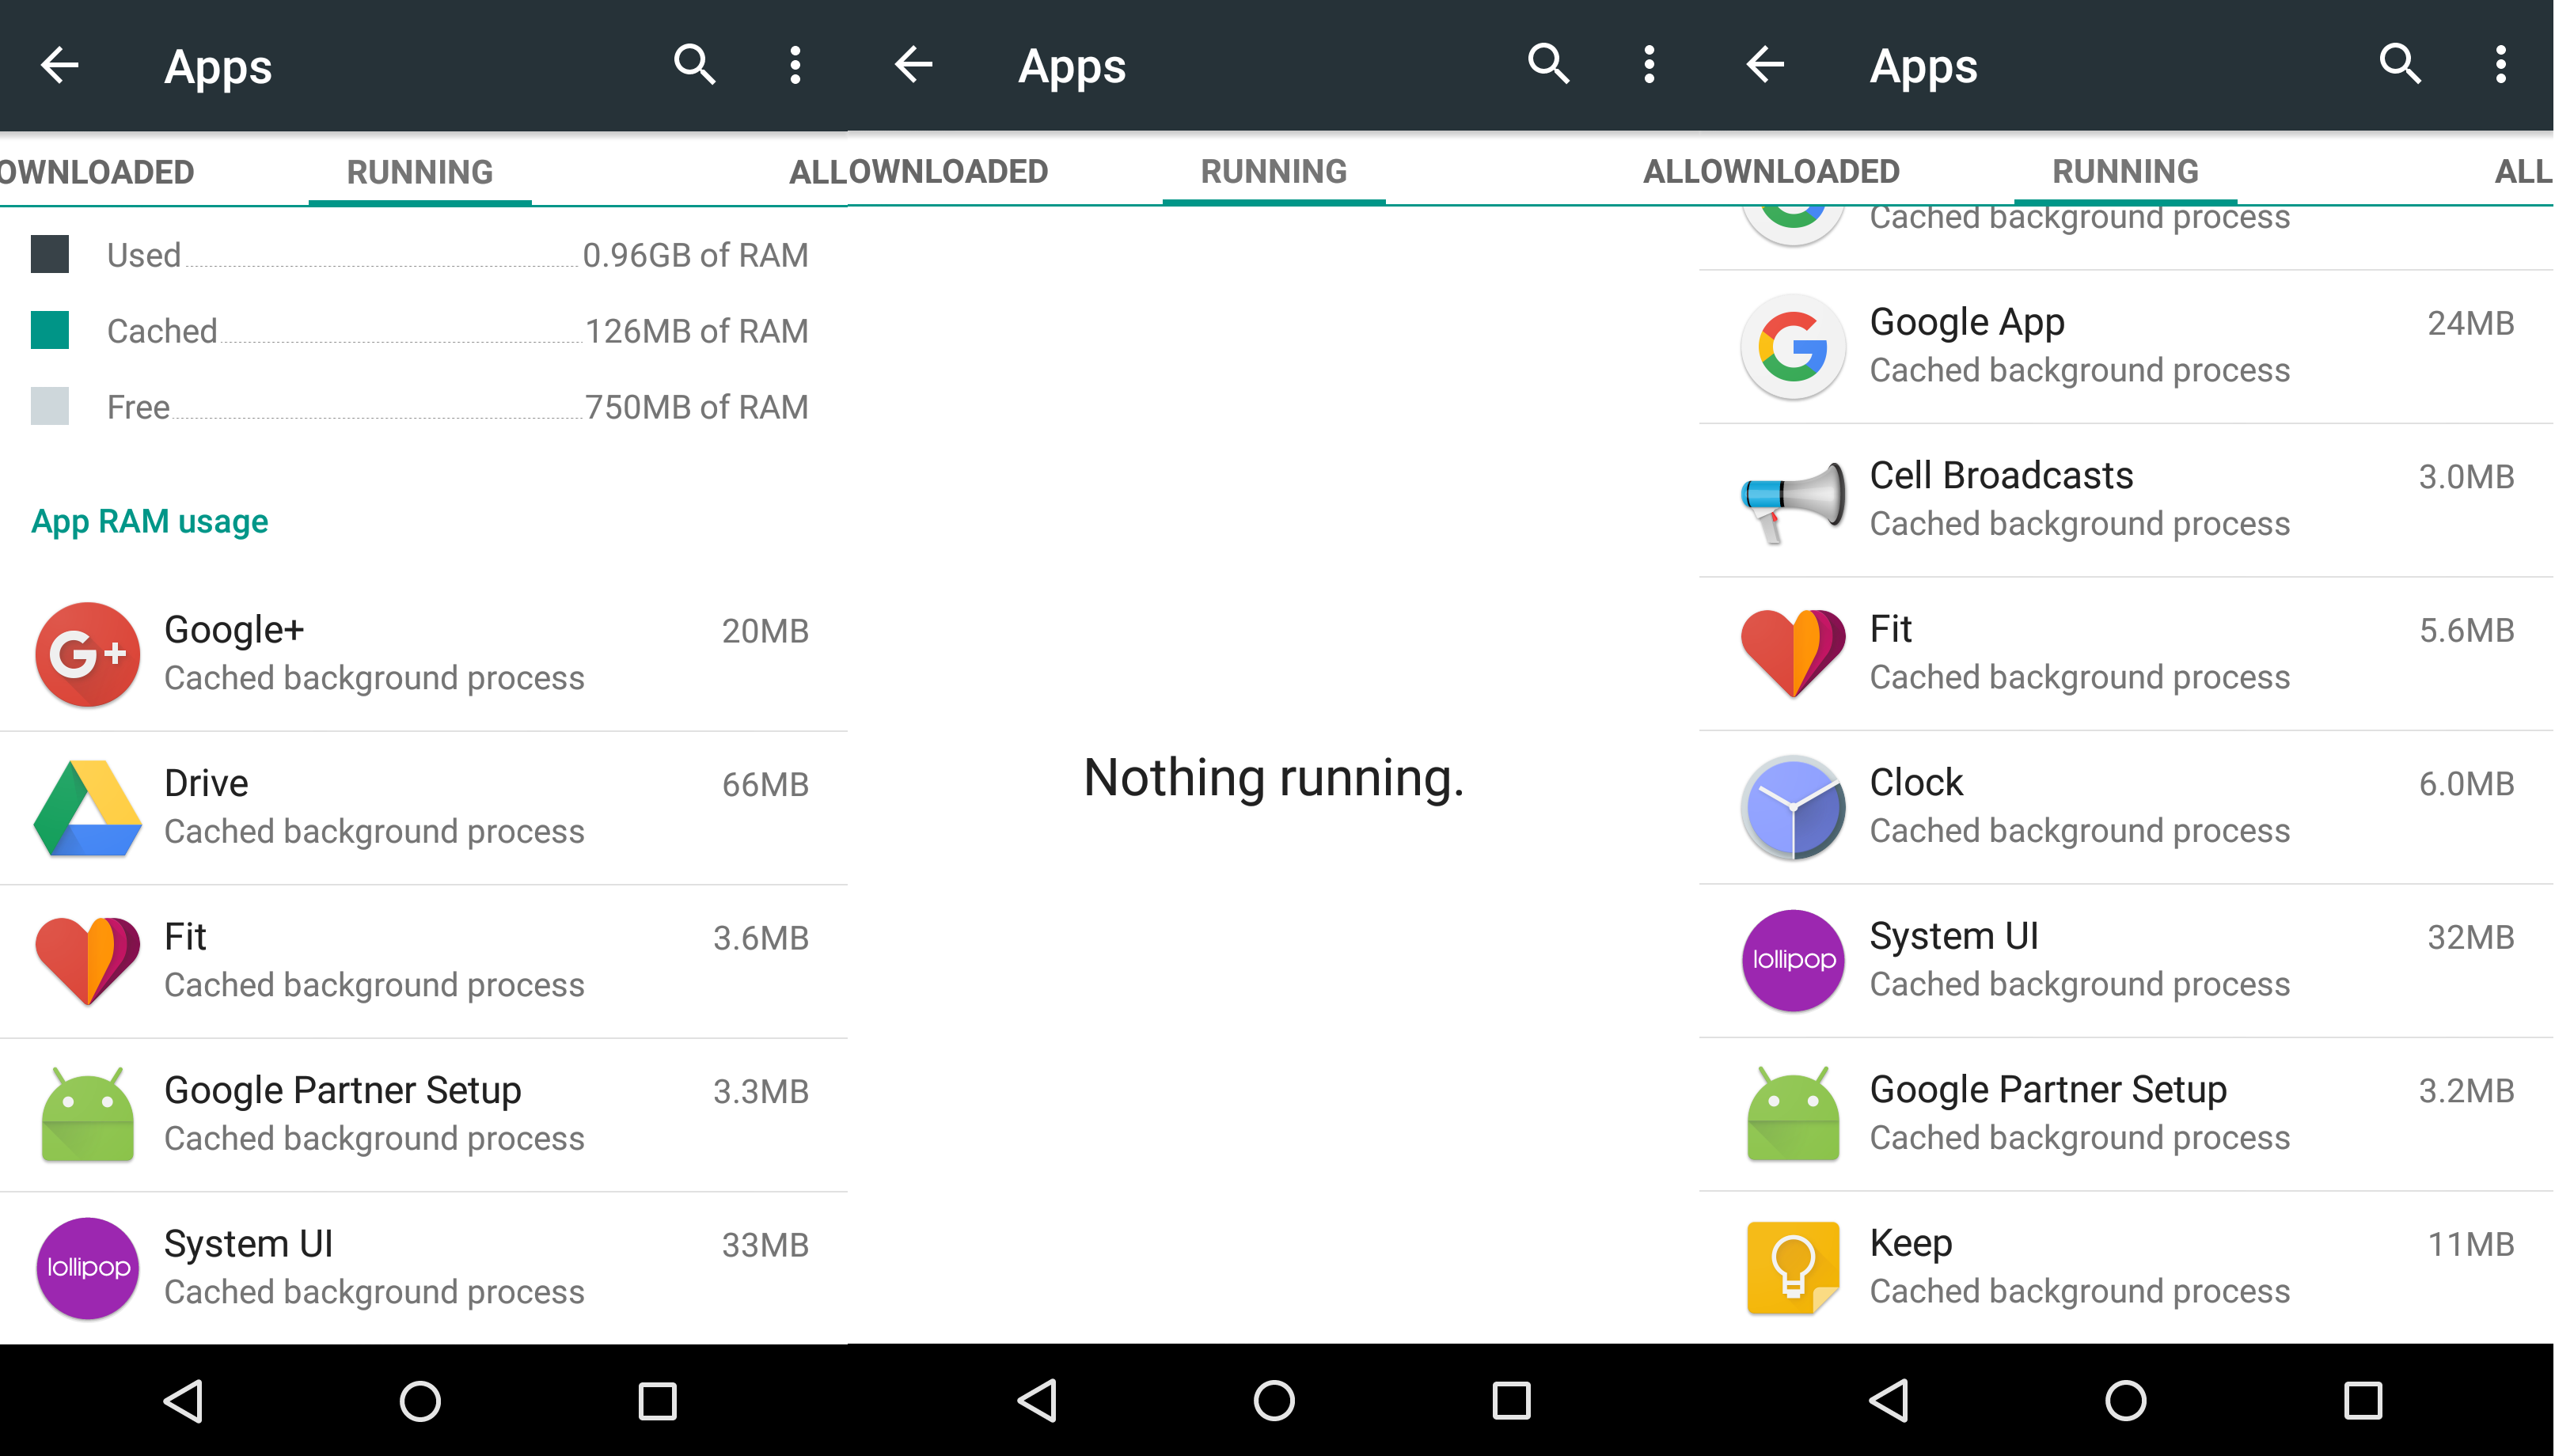
\includegraphics[width = 130mm]{images/stage123.png}
						\caption[CBP(s) before and after manual removal]
						{The leftmost image shows the snapshot of the CBP(s) before forceful deletion. After each and every CBP was removed manually, the screen displayed is shown in the middle image. The image farthest to the right shows the repopulated list of CBP(s), 3 minutes after the middle image was taken. This demonstrates Android's ability to utilize free RAM space and pro-actively cache CBP(s)}
					\end{figure}					
					
					This suggestes that Android recognizes that an under-utilized RAM is a waste of resource and pro-actively caches applications that were'nt in memory to begin with, as CBP(s). This is also the reason why task killer applications fell out of favor [33]. This demonstrates that not only does Android provide a mechanism to pro-actively cache applications in memory, it already does so. The applications suggested by the Hybrid CRA approach can be introduced into the memory as CBP(s) in the same way. This is discussed in future scope section. 

				\paragraph{Prioritizing Overall Cache}	
					The Hybrid CRA would involve storing as CBP(s), both default application components cached by Android's LRU scheme and the application components of the list of applications obtained from analyzing the user's Calendar. So the question now becomes, who gets kicked out when memory is running low? Since the applications inferred from user's contextual information do not have a recency associated with them, the LRU CRA cannot be applied over the overall list of CBP(s). A simple solution is to prioritize the CBP(s) obtained from the list of suggested applications over the default LRU based CBP(s) i.e. all the default CBP(s) are removed from memory before the CBP(s) cached as a result of context inference. There are two advantages to this approach:
					
					\begin{itemize}
						
						\item Only few applications are suggested by the context module.
						
							\begin{itemize}
								\item For instance, say the user has a Calendar entry that reads {\em Call Mom}. There will be two or at most three applications suggested by the context-module that would be potentially useful to the smart-phone user in the context of calling his mother. This makes it more convenient to target CBP(s) cached by the LRU scheme in case of low memory.
							\end{itemize}
							
						\item The probability of user requesting an application related to the Calendar event is quite high.
						
							\begin{itemize}
								
								\item This is due to the fact that a recorded event in a user's Calendar is highly likely to occur and the applications needed in this context have a higher chance of being utilized as opposed to CBP(s) cached by the LRU scheme.
								
								\item This is explored further in the future scope section where we discuss the relative probabilities of applications being used in conjunction with a Calendar event.
								
							\end{itemize}
								
					\end{itemize}  
					
		\subsection{Supplementary Data}
			We've talked about the fundamental metrics involved in measuring the efficiency of the APC, namely cache hits, cache misses and CHR. We explored potential candidates for serving as the CRA in managing the APC. There are other subtle measurements that are'nt as significant as the fundamental metrics but are important nonetheless as they shed light on certain attributes of the experiment. They are listed below:
			
			\begin{itemize}
				\item Number of Installed Applications
				\item Number of Unique Applications Requested (Clicked)
				\item Phone Model
				\item Android OS Version
			\end{itemize} 
			
			Depending on the value of the overall number of installed applications and the overall number of unique applications requested by the end-user, certain CRA(s) have an edge over the others. Phone model information is collected to see if there is any correlation between models and cache efficiencies. Some of the techniques used to gather context information are not possible in certain Android OS versions. We'll analyze the correlation between these fields and the efficiency of CRA(s) in the Section 5.  
			
	\section{Challenges}
		Now that we've established what the desired metrics are, let's examine some of the challenges in collecting them.  
		
		\subsection{Deciding Between System vs User Level Approach}
			Firstly, we need to determine whether to approach the problem from a user level perspective or not. Attempting to solve the problem i.e. collecting the aforementioned metrics at the user level would involve building Android applications to gather relevant data. On the other hand, approaching the problem from a system level would involve altering the source code of the Android OS (facilitated by AOSP) and recompiling it to build our own custom distribution, much like the CyanogenMod community [34]. It is easier to solve the problem (if possible) at the user level for two reasons:
			
			\begin{itemize}
				\item The complexity involved in altering OS source code is significantly higher compared to writing Android applications.
				\item It would be significantly harder to convince potential research volunteers to reboot their smart-phones with a custom distribution of the Android OS as opposed to asking them to install an Android application or two.
			\end{itemize}
			
			Given that it's beneficial to gather relevant data at the user level, we need to identify the complexities involved and determine whether they are solvable at the user level. In order to effectively determine which CRA is ideal for the APC, we need to identify whether the following problems can be approached from a user level perspective:
			
			\begin{itemize}
				\item Getting the list of processes currently in memory \checkmark
				\item Knowing when a new process is launched by the user \checkmark
				\item Reading the User's Calendar \checkmark
			\end{itemize} 
			
			We'll inspect in detail, why and how we need to solve these problems (and others) in the next section but the  '\checkmark' indicates that they are indeed solvable at the user level and do not require system level changes.
			
		\subsection{Getting Processes in Memory}
			Let's first address why it's necessary to get the list of processes that reside in memory. In our scenario, we are trying to determine the most efficient caching scheme amongst the following:
			
			\begin{itemize}
				\item LRU (Default)
				\item Pure Prediction (Applications will be cached solely based on context inference)
				\item LRU-Context Hybrid (or simply Hybrid)
			\end{itemize}
			
			In order to determine which scheme is most efficient, we need the ability to measure CHR data and by extension if and when a cache hit or miss occurs. We can only determine if a cache hit occurred if we had access to the list of processes in the cache i.e. the active processes and the CBP(s) in memory. The {\em ActivityManager} class in Android provides two relevant helper methods [35]:
			
			\begin{itemize}
				\item {\em getRunningTasks()}
				\item {\em getRunningAppProcesses()}
			\end{itemize} 
			
			Unfortunately, as of Android 5.0, it has become increasingly difficult to get a list of applications running in memory. {\em getRunningTasks()} has been deprecated and {\em getRunningAppProcesses()} has been killed (It only returns the requesting application rather than all applications running in memory). The documentation has'nt changed and Google is ignoring requests to either update the documentation or restore the original implementation. An alternate solution is to use the {\em UsageStatsManager} class [36]. However, it requires special permission from the user in the Settings application and some OEM (Original Equipment Manufacturers)(s) have removed this setting explicitly rendering this solution unreliable. The best solution involves using the ADB (Android Debug Bridge) shell to retrieve the desired information which can then be parsed into a suitable list of processes residing in memory. ADB is a versatile command line tool that enables communication with an emulator instance or a connected APMD. It is a client-server program that includes three components [37]:
			
			\begin{itemize}
				\item A client, which runs on the APMD. The client can be invoked from a shell by issuing an ADB command. Other Android tools can create ADB clients as well.
				\item A server, which runs as a background process on the APMD. The server manages communication between the client and the ADB daemon running on the APMD.
				\item A daemon, which runs as a background process on the APMD.
			\end{itemize}
			
			The ADB provides a Unix shell that can be used to run a variety of commands on the APMD. The command binaries are stored in the APMD's file system at {\em /system/bin/} [38]. We eventually obtain the list of processes residing in memory by running the {\em toolbox} command [42] in the shell. The Android {\em toolbox} command encapsulates the functionality of many common Linux commands (and some special Android commands) into a single binary [39]. Some of the commands provided by Toolbox are listed below (not an exhaustive list):
			
			\begin{itemize}
				\item cat, chmod, chown, cmp, cp
				\item ctrlaltdel, date, dd, df, dmesg
				\item toolbox, top, touch, umount
				\item ps, reboot, renice, rm, rmdir
			\end{itemize}
			
			Of these, we are most concerned with the {\em toolbox} and {\em ps} commands as they provide a direct window into the processes residing in memory. We use the following parameters with the {\em ps} command to get the desired process data:
			
			\begin{itemize}
				\item '-P': It shows the scheduling policy.
				\item '-p': It displays the priorities and niceness level.
				\item '-x': It shows system time in seconds
				\item '-c': It displays the CPU
			\end{itemize}
			
			With the help of {\em libsuperuser} library which provided a convenient framework to run shell commands [40] and Jared Rummler's {\em AndroidProcess} library that provided a framework to parse the process-related shell outputs [41], the following algorithm (Refer Algorithm 1) was written to obtain a list of processes residing in memory (active processes and CBP(s)). It is worth noting that this list corresponds to the list of processes displayed by the Settings application (Refer Figure 3-1) as part of the running applications and CBP screens, and that the Settings application has system privileges that third party Android applications don't.\\ 
			
			\begin{algorithm}[H]
				\SetAlgoLined
				\KwResult{LIST Process}
				
				INITIALIZE LIST Process - processes\\
				LIST String - stdout --- Shell.SH.run("toolbox ps -p -P -x -c")\\
				Integer myPid 		 --- android.os.Process.myPid()
				
				\For{String line : stdout}
				{
					INITIALIZE Process - process\\
					\eIf{process matches APP-ID-PATTERN}
					{
						\eIf{(process.ppid EQUAL TO myPid)\\ OR (process.name EQUAL TO "toolbox")}
						{
							CONTINUE
						}
						{
							ADD TO processes - process
						}
					}
					{
						CONTINUE
					}
				}
				
				RETURN processes;\\
			
			\caption[Algorithm to get list of processes in RAM]{In the above algorithm, {\em Process} is a custom data structure that parses the output format of the {\em toolbox ps} command. Its class structure is discussed in detail in Section 4.4. The {\em APP-ID-PATTERN} is a custom regular expression that maps to application ID patterns for the Android OS in versions 4.0 and above. Each process is added to a result list that is returned by the algorithm. Note that the requesting application represented by {\em myPid} (discussed in 4.4) and {\em toolbox} related processes represented by process names that match {\em toolbox}, are'nt added to the result.}
			\end{algorithm}			
			
		\subsection{Obtaining the Foreground Application}
			In order to update the CHR metric, we need the ability to detect new cache hits and cache misses. A new cache hit/miss occurs when there are new application requests i.e. changes in the foreground application. Before we analyze how to detect change in the foreground application, we first need a way to obtain the current foreground application. Had we approached this problem at the system level, we could've made use of system level privileges such as listening to a new screen-touch by the user and detecting which application was  launched but this is not possible from a third party user-level application. Fortunately, there is a workaround to detecting the foreground application at the user level. We obtain every process currently running in memory and through a process of elimination, obtain the foreground application. To elaborate, the foreground application has certain unique properties in its process name, UID (Unique Identifier) and other fields, that can be exploited to eliminate processes that are not associated with the current foreground application. The following   algorithm (Refer Algorithm 2) illustrates this process.
			
			\begin{algorithm}[H]
				\SetAlgoLined
				\KwResult{Foreground Application}
				
				INITIALIZE LIST {\em files} --- LIST {\em /proc} File\\
				\For{File file : files}
				{
					\If{file IS A DIRECTORY}{CONTINUE}
					
					{\em pid --- file.getName()}\\
					{\em cgroup} --- FILE READ ({\em /proc/\%d/cgroup})\\
					{\em cpuSubSystem, cpuAccountSubSystem --- cgroup}\\
					
					\If{cpuAccountSubSystem ENDS WITH pid OR cpuSubSystem ENDS WITH bg\_non\_interactive}{CONTINUE}
					
					{\em cmdline} --- FILE READ ({\em /proc/\%d/cmdline})\\
					{\em uid} --- PARSE FROM {\em cpuAccountSubSystem}\\
					
					\If{cmdline CONTAINS com.android.systemui OR uid BETWEEN 1000 AND 1038}{CONTINUE}
					
					{\em oomAdj} --- FILE READ ({\em /proc/\%d/oom\_score\_adj})\\
					{\em oomScore} --- FILE READ ({\em /proc/\%d/oom\_score})\\
					
					\If{LOWEST oomScore AND oomAdj EQUAL TO 0}{RETURN cmdline}
				}
				
				\caption[Algorithm to get current foreground application]{This algorithm obtains the current foreground process i.e. the process associated with the application that the user is interacting with.}
			\end{algorithm}
			
			Firstly, all files with path {\em /proc} are obtained and each iterated over, to find the foreground application. We eliminate file directories as these are of no concern to us. If the CPU account sub-system ends with {\em pid}, it's not an application process and is thus eliminated. Similarly, if the CPU sub-system ends with {\em bg\_non\_interactive}, it's a background process and is eliminated as well. The application stored in {\em cmdline} is a potential candidate for the foreground application and is the right choice as long as it clears four more hurdles:
			
			\begin{itemize}
				\item {\em cmdline} does not contain {\em com.android.systemui}
				\item {\em uid} does not lie between 1000 and 1038
				\item {\em oomAdj} i.e. the OOM (Out Of Memory) adjustment level [43] equals 0
				\item {\em oomScore} is the lowest among all iterated values
			\end{itemize}
			
			If {\em cmdline} contains {\em com.android.systemui} or if {\em uid} lies between 1000 and 1038, it's a system application and is thus eliminated from consideration. The crucial attribute of the foreground application is that it has the lowest OOM score of all applications. When the Android OS is running too low on memory, it is the job of the Linux OOM killer [44] to sacrifice one or more processes in order to free up memory for the system when all else fails. A low OOM score indicates that the process is less likely to be killed and that it is lower on the OOM killer's radar. It quite intuitive that the process with the lowest OOM score would be the foreground process as it is of paramount importance not to remove the process, the end-user is interacting with, unless it's the very last resort. This unique property of the foreground process enables us to distinguish it from the rest of the pool. 
			
		\subsection{Updating the Statistics}
			 So far, we've established ways to collect the list of processes in memory and the foreground application. The next step is to figure out a way to update the metrics as and when the user requests new applications. The rate at which the end-user toggles between applications varies from person to person. It also depends on the level of usage. For instance, there are times when the end-user is actively using their APMD and others when the APMD is idle or is switched off. Therefore it's hard to predict when there could be a potential change in the foreground application. There is no inherent mechanism for user-level applications to detect third party application launches (That privilege is reserved for system level processes). Therefore, our solution comprises of starting a service [8] that retrieves the current foreground process (Refer Algorithm 2) and the current list of processes residing in memory (Refer Algorithm 1) every second. If there is a change detected in the foreground process (compared to the last second), then the cache metrics are updated. The time interval of one second is chosen as it deemed to be reasonably accommodative of the average time it takes an end-user to switch from one application to another. This is further discussed in the Points of Weakness section. The design of the service and the corresponding application is discussed in sections 4.4 and 4.5. The following algorithm (Refer Algorithm 3) illustrates the process of updating the cache metrics.\\     
			 
		 	\begin{algorithm}[H]
		 		\SetAlgoLined
		 		\KwResult{Update Cache Metrics}
		 				 		
		 		\For{EACH SECOND}
		 		{	
		 			{\em newForegroundApp --- getNewForegroundApp()}\\
		 			{\em currentListOfProc --- getListOfProcesses()}\\	 			
		 			\If{newForegroundApp EQUALS oldForegroundApp}{CONTINUE}
		 			\eIf{oldListOfProc CONTAINS newForegroundApp}{cacheHit++}{cacheMiss++}
		 			{\em updateMetrics()}\\
		 			{\em oldListOfProc --- newListOfProc}\\
		 			{\em oldForegroundApp --- newForegroundApp}		 			
		 		}
		 		
		 		\caption[Algorithm to update cache metrics]{This algorithm retrieves the foreground application and checks if it has changed since the last second. If it has, it verifies whether it was a cache hit or a cache miss and updates the cache metrics. Finally, it updates the old foreground application and the previous list of processes to the current one so that the next iteration uses these values as the base.}
		 	\end{algorithm}

		\subsection{Backing Up the Data}
			Previously, we discussed the mechanism by which the background service updates the cache metrics. The other aspect of this issue is storing this data. Before we inspect how to store the data, let's discuss the necessity for such a provision. Our background service is designed to run throughout the duration of the experiment and retrieve the foreground application and the list of processes in memory every second. This results in it's OOM score increasing i.e. it's likelihood of getting killed by the Linux OOM killer [44] which would result in a loss of data. It is worth noting that the OOM killer selects the {\em best} process to kill which is decided by the combination of how long a process has been running and how much memory would be released if the process is killed. Even though our process scores poorly on the time duration aspect, it takes up relatively low memory compared to some of the other common background processes (Refer Figure 3-6).

			\begin{figure}[h]
				\centering
				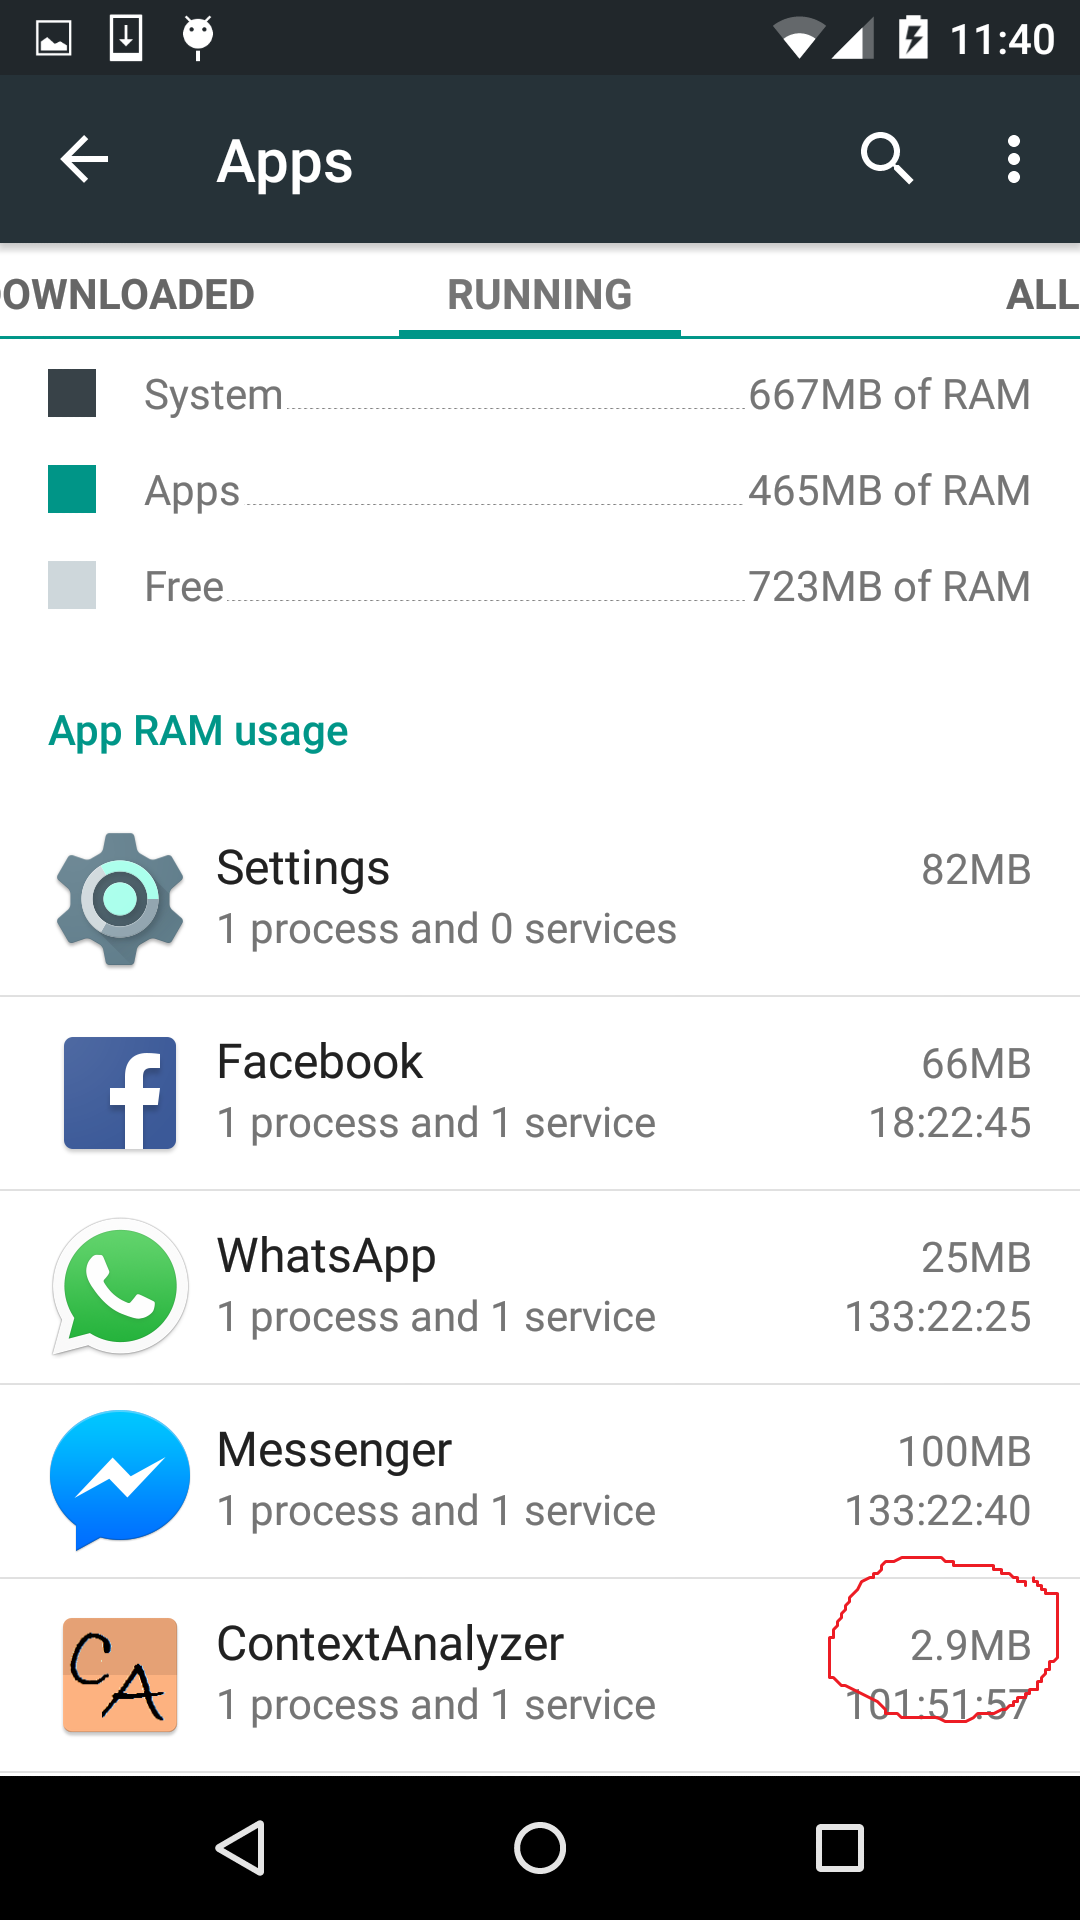
\includegraphics[width = 70mm]{images/lowMemory.png}
				\caption[Memory Occupied by the Background Service]{CacheAnalyzer is an application that collects the default (LRU) cache metrics. The service mentioned in the diagram is the background service that updates the metrics every second. We'll discuss the design of this application in Section 4.4 but it's worth noting here that the memory footprint of the application is quite low. This is not to suggest that it won't get killed by the OOM killer, which is why we're backing the data up.}
			\end{figure} 

			Android provides several options for saving persistent application data. There are five ways to accomplish this task [45]:
			
			\begin{itemize}
				\item Shared Preferences - It is used in cases where primitive data needs to be stored in Key Value pairs.
				\item Internal Storage - It is used to store private data on device memory.
				\item External Storage - It is used to store public data on shared external storage
				\item SQLite Databases - They are used to store structured data in a relational database.
				\item Network Connection - It is used to store data over the Internet.
			\end{itemize}
			
			For our scenario, Internal Storage is the best fit as it keeps the data private to the application and since the data is quite primitive (cache hits and misses), we do not need SQLite databases or network connections. The data is written to a file every minute. That way, we don't have to constantly perform I/O operations from the service and in the worst case scenario, fifty nine seconds of Cache data would be lost which is relatively a small amount of time. Algorithm 3 can be tweaked to incorporate the file write operation (Refer Algorithm 4).
			
			\begin{algorithm}[H]
				\SetAlgoLined
				\KwResult{Update Cache Metrics AND Write to File}
				
				\For{EACH SECOND}
				{	
					...\\
					...\\
					{\em updateMetrics()}\\
					\If{END OF MINUTE}{ writeMetricsToFile()}
					...\\
					...\\	
				}
				
				\caption[Modified Update Metrics Algorithm]{In addition to updating the metrics every second, it also writes the data to internal storage every minute. Any time the application is closed and launched again the metrics are initialized with the values in file.}
			\end{algorithm}
			
		\subsection{Reading the User's Calendar}
			To compute the CHR of the Hybrid CRA approach, we need the ability to obtain the list of events from the user's calendar and the ability to parse that information to come up with a list of suggested applications. We'll discuss the parsing aspect in the next segment and focus on finding a way to read the user's calendar. The solution to this problem is quite simple, Google provides a public API (Application Programming Interface) [46] to obtain access to the user's calendar information, including the list of events. This operation does'nt have to be carried out with the same frequency as reading the list of processes in memory or obtaining the foreground application. In our solution, we query the calendar every four hours (for events occurring in that four hour period) and feed the data (events list) into a module that parses the information and produces a suggested list of applications (Refer Algorithm 5). 
			
			\begin{algorithm}[H]
				\SetAlgoLined
				\KwResult{Update Cache Metrics, Write to File AND Update List of Suggested Applications}
				
				\For{EACH SECOND}
				{	
					...\\
					...\\
					{\em updateMetrics()}\\
					\If{END OF MINUTE}{ writeMetricsToFile()}
					\If{END OF 4 HOURS}{updateListOfSuggestedApplications()}
					...\\
					...\\	
				}
				
				\caption[Update Suggested Applications List]{In addition to updating the metrics every second and writing them to file every minute, it also updates the list of applications suggested by the Calendar Parser (discussed in next segment)}
			\end{algorithm}
			
			The following algorithm (Algorithm 6) illustrates our implementation of the module that queries the user's calendar.
			
			\begin{algorithm}[H]
				\SetAlgoLined
				\KwResult{Get List of Events from Calendar}
				INITIALIZE List {\em result}\\
				List {\em allEvents} ---  QUERY {\em content://com.android.calendar/events}\\
				\For{EACH event IN allEvents}
				{	
					\If{event.startTime() IS WITHIN 4 hours FROM NOW}{result.add(event)}
				}
				RETURN result
				\caption[Algorithm to read user's calendar]{This algorithm obtains all events in the user's calendar that start within 4 hours from the time of the algorithm invocation. Since this algorithm is invoked every four hours, every event in the user's calendar is parsed although it's worth noting that once read, a change in the event details is not translated to the application. This is discussed further in the Points of Weaknesses section.}
			\end{algorithm}
						
		\subsection{Parsing the Calendar Information}
			We've examined the mechanism behind reading the user's calendar, thereby solving one half of the puzzle. The other half is utilizing this information to compute the Hybrid CRA's metrics. In order to achieve that, we need to build a module that parses the list of events obtained from reading the calendar and produces a suggested list of applications. Every event in the user's calendar is split into individual keywords and a predetermined mapping between keywords and applications builds the list of suggested applications. For instance the keyword {\em mail} is associated with the {\em GMail} application, among others. This mapping is determined by a combination of three things:
			
			\begin{itemize}
				\item The suggestions from the Google Play Store [48] when searched with the keyword.
				\item The number of downloads among competing applications for the same keyword.
				\item Popularity of the applications in United States of America (USA) [47]. 
			\end{itemize}

			To elaborate, when the Play Store was searched with the keyword {\em skype}, Skype application was the top result. Once it is verified that Skype is part of the installed applications [49], it is added to the list of suggested applications. It is worth noting that most of the suggested applications are present by default on Android (such as GMail, Hangouts, Docs to list a few) and the only applications that are checked against the list of installed applications are highly popular applications [47]. Additionally, if there are no events in the user's calendar for the four hour period, then the list of suggested applications is populated with the ten most popular Android applications in USA [47]. Theoretically it seems likely that the user might use the applications suggested by Google's application search engine, for a particular keyword. However, it remains to be seen whether the suggested applications result in cache hits and by extension a better caching scheme. We'll analyze this data in Chapter 5.   
		

\chapter{Experiment Setup and Application Design}
	
	\section{Introduction}
		In the previous chapter, we examined the metrics we needed to analyze the best caching scheme for the APC. We looked into some of the common CRA(s) and analyzed some of the challenges in collecting the metrics needed to determine if contextual information can help better the CHR of the Hybrid approach. To analyze the efficiencies of the default LRU and the Hybrid approaches, two Android applications namely {\em CacheAnalyzer} and {\em ContextAnalyzer} were written and installed in the APMD(s) of research volunteers. In this chapter, we'll address the details of the experiment and analyze the design of these two Android applications. 
		
	\section{Eligibility for Volunteers}
		The following criteria had to be met to qualify as a research volunteer:
		
		\begin{itemize}
			\item The volunteer must own an APMD with Android OS version greater than 5.0 (Lollipop and above).
			\item The volunteer must be willing to install two third party applications on their APMD for the duration of a week.
		\end{itemize}
		
		The algorithm that obtains the list of processes currently residing in memory and the algorithm that retrieves the current foreground application do not apply to Android OS versions below 5.0, hence the necessity for APMD(s) with OS versions that are Lollipop and above.
		
		\subsection{Addressing Privacy Concerns}
			Since the research volunteers had to install two third party applications ({\em CacheAnalyzer} and {\em ContextAnalyzer}), it was crucial to address any privacy concerns that arose. In order to gain the trust of the volunteers, we adopted a policy of full transparency and took the following measures:
			
			\begin{itemize}
				\item We fully explained to each volunteer, the nature of the data we were collecting i.e. cache metrics.
				\item We open sourced both Android applications [50][51] in case the volunteers wanted to verify that there were no nefarious activities going on in the background.
				\item We did not automatically store the cache metrics in a server. Instead, we asked the volunteers to send us the data in order to convey the message that we were'nt collecting any private data that the volunteers were'nt aware of.
			\end{itemize}
			
			Although the aforementioned points address the privacy issues, we realize that divulging the nature of the experiment has the potential to bias the volunteers in their APMD usage. We explore this aspect in detail in the Points of Weaknesses section. 
	
	\section{Process and Duration of Experiment}
	
	\section{Cache Analyzer Design}
	
	\section{Context Analyzer Design}
	
	\section{Tools, Version Control and APK}
		
		\subsection{Android Studio}
		
		\subsection{Git}
		
		\subsection{Third Party APK(s)}

\chapter{Data Analysis and Results}
	
	\section{Introduction}
	
	\section{Phase A Data}
	
	\section{Phase B Data}
	
	\section{Default Approach Metrics}
	
	\section{Pure Prediction Approach Metrics}
	
	\section{Hybrid Approach Metrics}
	
	\section{Factors Influencing Variation In Data}
		
		\subsection{Android Version and Phone Model}
		
		\subsection{Number of Applications Installed}
		
		\subsection{Number of Applications Used}
		
		\subsection{User Bias}
		
		\subsection{User Demographics}
	
	\section{Points of Weakness}		
		
		\subsection{Constant Change in Calendar events}
		
		\subsection{List from Google Drive}
		
		\subsection{Slight Increase in Battery Consumption}
		
		\subsection{Divulging the Nature of the Experiment}
		
\chapter{Scope for Future Work}
		
	\section{Introduction}
		
	\section{Improving Context Analysis}
		
		\subsection{Machine Learning in Calendar Parsing}
		
		\subsection{Calendar Parser - LFU Hybrid}
		
		\subsection{Other Ways of Gathering User Behavior Data}
		
		\subsection{Custom Priorities in Hybrid Cache}
			% If 'call' was parsed from Calendar, then dialer app is high priority followed by LRU followed by other call apps.
			
			%Previous point - We can use machine learning to come up with custom priorities 
	\section{Alternate Ways of Using the Contextual Information}
			
		\subsection{Switching to Silent Mode}
			
		\subsection{Disabling Texting at High Speeds}
		
	\section{Implementing the Hybrid Cache}

\chapter{Conclusion}		

%XXXXXXXXXXXXXXXXXXXXXXXXXXXXXXXXXXXXXXXXXXXXXXXXXXXXXXXXXXXXXXXXXXXX
%XXXXXXXXXXXXXXXXXXXXXXXXXXXXXXXXXXXXXXXXXXXXXXXXXXXXXXXXXXXXXXXXXXXX
%XXXXXXXXXXXXXXXXXXXXXXXXXXXXXXXXXXXXXXXXXXXXXXXXXXXXXXXXXXXXXXXXXXXX
%XXXXXXXXXXXXXXXXXXXXXXXXXXXXXXXXXXXXXXXXXXXXXXXXXXXXXXXXXXXXXXXXXXXX

%--------+----------------------------------------------------------+
%        |  \myreferences{}                          (CONDITIONAL)  |
%        |                                                          |
%        |  See section 3.18 of "Read_Me_First_(v12).pdf"           |
%        |                                                          |
%        |  That section of the READ ME file describes two options  |
%        |  for listing the works cited in your document: first,    |
%        |  manually entering your list of references and, second,  |
%        |  using BibTeX to generate that list.                     |
%        |                                                          |
%        |  1) If you manually enter your reference list, first     |
%        |     include the \myreferences command, as illustrated    |
%        |     below.  Second, use the "referencelist" environment  |
%        |     described below.  For this, note that the UT Manual  |
%        |     requires double-spacing *between* references in      |
%        |     that list. However, it also states that *within*     |
%        |     individual references the spacing may be single- or  |
%        |     double-spaced.  Because of this, UThesis provides    |
%        |     two options for the "referencelist" environment:     |
%        |                                                          |
%        |            \begin{referencelist}{ENTER OPTION HERE}      |
%        |            \item ...                                     |
%        |            \end{referencelist}                           |
%        |                                                          |
%        |     a. Replacing "ENTER OPTION HERE" above with the      |
%        |        text "single" will generate a reference list      |
%        |        with single-spaced entries in that list but       |
%        |        double-spacing between those entries. An example  |
%        |        of this is provided below.                        |
%        |     b. Alternatively, using the "double" option will     |
%        |        generate a list with double-spaced entries and    |
%        |        double-spacing between entries. An example of     |
%        |        this is also provided below.                      |
%        |                                                          |
%        |     Note that input to these options is case sensitive   |
%        |     and the default setting is the "double" option.      |
%        |                                                          |
%        |  2) If you instead choose to use BibTeX to generate the  |
%        |     reference list, then you *cannot* include either     |
%        |     the "\myreferences" command or the "referencelist"   |
%        |     environment in your document. In this case you must  |
%        |                                                          |
%        |     a. delete the \myreferences command and the two      |
%        |        examples of the "referencelist"  environment      |
%        |        below;                                            |
%        |     b. then you must add and locate appropriately all    |
%        |        necessary BibTeX commands within your document    |
%        |        (e.g., \bibliographystyle{}, \citationstyle{},    |
%        |        \bibliography{}, etc.).                           |
%        +----------------------------------------------------------+

\myreferences

\begin{referencelist}{single}
	
	\item \textbf{[1]} ``The Android Source Code''
	\\\emph{http://source.android.com/source/index.html}, October 2015. 
	Online; Last Accessed: October 22, 2015.	
	
	\item \textbf{[2]} ``The Most Popular Smartphone Operating Systems Globally,''
    \\\emph{http://www.lifehacker.com.au/2014/09/the-most-popular-smartphone-operating-systems-around-the-world/}, September 2014. 
    Online; Last Accessed: October 22, 2015.
	
	\item \textbf{[3]} ``Android System Architecture''
	\\\emph{https://mahalelabs.files.wordpress.com/2013/03/androidstack-1.jpg}, March 2013. 
	Online; Last Accessed: October 22, 2015. 
		
	\item \textbf{[4]} ``Best custom ROMs for the Samsung Galaxy S2''
	\\\emph{http://www.cnet.com/uk/how-to/best-custom-roms-for-the-samsung-galaxy-s2/}, April 2012. 
	Online; Last Accessed: October 22, 2015. 
		
	\item \textbf{[5]} ``Widgets | Android Developers''
	\\\emph{http://developer.android.com/design/patterns/widgets.html}, October 2015. 
	Online; Last Accessed: October 22, 2015.
		
	\item \textbf{[6]} ``Application Fundamentals | Android Developers''
	\\\emph{http://developer.android.com/guide/components/fundamentals.html}, October 2015. 
	Online; Last Accessed: October 22, 2015.
		
	\item \textbf{[7]} ``Activities | Android Developers''
	\\\emph{http://developer.android.com/guide/components/activities.html}, October 2015. 
	Online; Last Accessed: October 22, 2015.					     

	\item \textbf{[8]} ``Services | Android Developers''
	\\\emph{http://developer.android.com/guide/components/services.html}, October 2015. 
	Online; Last Accessed: October 22, 2015.
	
	\item \textbf{[9]} ``Wikimedia Upload''
	\\\emph{http://www.extremetech.com/wp-content/uploads/2015/04/MooresLaw2.png}, October 2015. 
	Online; Last Accessed: October 22, 2015.
	
	\item \textbf{[10]} ``A Brief History of Android Phones''
	\\\emph{http://www.cnet.com/news/a-brief-history-of-android-phones/}, August 2011. 
	Online; Last Accessed: October 22, 2015.
	
	\item \textbf{[11]} ``GSM Arena''
	\\\emph{http://www.gsmarena.com/t\_mobile\_g1-2533.php}, October 2008. 
	Online; Last Accessed: October 22, 2015.
	
	\item \textbf{[12]} ``Nexus 6P''
	\\\emph{http://www.androidcentral.com/nexus-6p}, October 2015. 
	Online; Last Accessed: October 22, 2015.
	
	\item \textbf{[13]} ``Phone Egg | LG T585''
	\\\emph{http://us.phonegg.com/phone/4783-LG-T585}, November 2013. 
	Online; Last Accessed: October 22, 2015.		
	
	\item \textbf{[14]} ``Android PSA: Stop Using Task Killer Apps''
	\\\emph{http://phandroid.com/2011/06/16/android-psa-stop-using-task-killer-apps-now/}, June 2011. 
	Online; Last Accessed: October 22, 2015.
	
	\item \textbf{[15]} ``Processes and Application Life Cycle''
	\\\emph{http://developer.android.com/guide/topics/processes/process-lifecycle.html}, October 2015. 
	Online; Last Accessed: October 22, 2015.
	
	\item \textbf{[16]} ``Managing Your App's Memory''
	\\\emph{http://developer.android.com/training/articles/memory.html}, October 2015. 
	Online; Last Accessed: October 22, 2015.	
	
	\item \textbf{[17]} ``Theodore Johnson, Dennis Shasha - A Low Overhead High Performance Buffer Management Replacement Algorithm''
	\\\emph{http://www.vldb.org/conf/1994/P439.PDF}, January 1994. 
	Online; Last Accessed: October 22, 2015.	
		
	\item \textbf{[18]} ``Hannu Verkasalo - Contextual patterns in mobile service usage''
	\\\emph{http://lib.tkk.fi/Diss/2009/isbn9789512298440/isbn9789512298440.pdf}, March 2008. 
	Online; Last Accessed: October 23, 2015.
			
	\item \textbf{[19]} ``Mika Raento, Antti Oulasvirta, Renaud Petit, and Hannu Toivonen - ContextPhone: A Prototyping Platform for Context-Aware Mobile Applications''
	\\\emph{http://dl.acm.org/citation.cfm?id=1070628}, May 2005. 
	Online; Last Accessed: October 23, 2015.
	
	\item \textbf{[20]} ``Anind K.~Dey, Gregory D.~Abowd and Daniel Salber - A Conceptual Framework and a Toolkit for Supporting the Rapid Prototyping of Context-Aware Applications ''
	\\\emph{http://www.cc.gatech.edu/fce/ctk/pubs/HCIJ16.pdf}, January 2001. 
	Online; Last Accessed: October 23, 2015.
	
	\item \textbf{[21]} ``Sensors | Android Developers''
	\\\emph{http://developer.android.com/guide/topics/sensors/sensors\_overview.html}, October 2015. 
	Online; Last Accessed: October 23, 2015.
	
	\item \textbf{[22]} ``Elaine Shi, Yuan Niu, Markus Jakobsson, and Richard Chow - Implicit Authentication through Learning User Behavior''
	\\\emph{markus-jakobsson.com/wp-content/uploads/2010/11/ShiNiuJakobssonChow2010.pdf}, November 2010. 
	Online; Last Accessed: October 23, 2015.

	\item \textbf{[23]} ``Alan Jay Smith - Design of CPU Cache Memories''
	\\\emph{http://www.eecs.berkeley.edu/Pubs/TechRpts/1987/CSD-87-357.pdf}, August 1987. 
	Online; Last Accessed: October 23, 2015.
			
	\item \textbf{[24]} ``Cache Hit | Techopedia''
	\\\emph{https://www.techopedia.com/definition/6306/cache-hit}, October 2015. 
	Online; Last Accessed: October 23, 2015.
	
	\item \textbf{[25]} ``Cache Miss | Techopedia''
	\\\emph{https://www.techopedia.com/definition/6308/cache-miss}, October 2015. 
	Online; Last Accessed: October 23, 2015.	
									
	\item \textbf{[26]} ``Najeeb A. Al-Samarraie - And Page Replacement Algorithms: Anomaly Cases''
	\\\emph{http://www.iasj.net/iasj?func=fulltext\&aId=50712}, January 2003. 
	Online; Last Accessed: October 23, 2015.
										
	\item \textbf{[27]} ``LRU Replacement Policy''
	\\\emph{https://www.seas.upenn.edu/~cit595/cit595s10/handouts/LRUreplacementpolicy.pdf}, October 2015. 
	Online; Last Accessed: October 24, 2015.
	
	\item \textbf{[28]} ``Hong-Tai Chou, David J. Dewitt - An Evaluation of Buffer Management Strategies for Relational Database Systems''
	\\\emph{http://www.vldb.org/conf/1985/P127.PDF}, October 1985. 
	Online; Last Accessed: October 24, 2015.
	
	\item \textbf{[29]} ``Shaul Dar, Michael J.~Franklin, Bjorn T.~Jonsson, Divesh Srivastava, Michael Tan - Semantic Data Caching and Replacement''
	\\\emph{http://www.vldb.org/conf/1996/P330.PDF}, October 1996. 
	Online; Last Accessed: October 24, 2015.
	
	\item \textbf{[30]} ``Donghee Lee, Member, IEEE, Jongmoo Choi, Member, IEEE, Jong-Hun Kim, Member, IEEE,
	Sam H. Noh, Member, IEEE, Sang Lyul Min, Member, IEEE, Yookun Cho, Member, IEEE, and
	Chong Sang Kim, Senior Member, IEEE - LRFU: A Spectrum of Policies that
	Subsumes the Least Recently Used and
	Least Frequently Used Policies''
	\\\emph{http://u.cs.biu.ac.il/~wiseman/2os/lru/lrfu.pdf}, December 2001. 
	Online; Last Accessed: October 24, 2015.

	\item \textbf{[31]} ``An Upper Limit For Apps? New Data Suggests Consumers Only Use Around Two Dozen Apps Per Month''
	\\\emph{http://techcrunch.com/2014/07/01/an-upper-limit-for-apps-new-data-suggests-consumers-only-use-around-two-dozen-apps-per-month/}, July 2014. 
	Online; Last Accessed: October 24, 2015.
											
	\item \textbf{[32]} ``ARM Documentation''
	\\\emph{http://infocenter.arm.com/help/index.jsp?topic=/com.arm.doc.set.cortexr/index.html}, July 2014. 
	Online; Last Accessed: October 24, 2015.

	\item \textbf{[33]} ``Does Your Android Device Really Need a Task Killer?''
	\\\emph{http://www.technorms.com/40664/android-task-killer-apps}, September 2014. 
	Online; Last Accessed: October 24, 2015.
											
	\item \textbf{[34]} ``CyanogenMod''
	\\\emph{http://www.cyanogenmod.org/}, October 2015. 
	Online; Last Accessed: October 24, 2015.
											
	\item \textbf{[35]} ``Activity Manager | Android Developers''
	\\\emph{http://developer.android.com/reference/android/app/ActivityManager.html}, October 2015. 
	Online; Last Accessed: October 24, 2015.
	
	\item \textbf{[36]} ``Usage Stats Manager | Android Developers''
	\\\emph{https://developer.android.com/reference/android/app/usage/UsageStatsManager.html}, October 2015. 
	Online; Last Accessed: October 24, 2015.																			

	\item \textbf{[37]} ``Android Debug Bridge | Android Developers''
	\\\emph{http://developer.android.com/tools/help/adb.html}, October 2015. 
	Online; Last Accessed: October 24, 2015.

	\item \textbf{[38]} ``ADB Shell Commands | Android Developers''
	\\\emph{http://developer.android.com/tools/help/shell.html}, October 2015. 
	Online; Last Accessed: October 24, 2015.
	
	\item \textbf{[39]} ``Android Toolbox''
	\\\emph{http://elinux.org/Android\_toolbox}, October 2015. 
	Online; Last Accessed: October 24, 2015.
	
	\item \textbf{[40]} ``Chainfire | Github | libsuperuser''
	\\\emph{https://github.com/Chainfire/libsuperuser}, October 2015. 
	Online; Last Accessed: October 24, 2015.
	
	\item \textbf{[41]} ``Jared Rummler | Github | AndroidProcesses''
	\\\emph{https://github.com/jaredrummler/AndroidProcesses}, October 2015. 
	Online; Last Accessed: October 24, 2015.

	\item \textbf{[42]} ``toolbox | Github''
	\\\emph{https://github.com/android/platform\_system\_core/tree/master/toolbox}, October 2015. 
	Online; Last Accessed: October 24, 2015.	
					
	\item \textbf{[43]} ``Low RAM Configuration | Android Source Code''
	\\\emph{https://source.android.com/devices/tech/config/low-ram.html}, October 2015. 
	Online; Last Accessed: October 24, 2015.
						
	\item \textbf{[44]} ``OOM Killer''
	\\\emph{http://linux-mm.org/OOM\_Killer}, October 2015. 
	Online; Last Accessed: October 24, 2015.
	
	\item \textbf{[45]} ``Storage Options | Android Developers''
	\\\emph{http://developer.android.com/guide/topics/data/data-storage.html}, October 2015. 
	Online; Last Accessed: October 24, 2015.

	\item \textbf{[46]} ``Calendar Provider | Android Developers''
	\\\emph{http://developer.android.com/guide/topics/providers/calendar-provider.html}, October 2015. 
	Online; Last Accessed: October 24, 2015.

	\item \textbf{[47]} ``These are the 25 most popular mobile apps in America''
	\\\emph{http://qz.com/481245/these-are-the-25-most-popular-2015-mobile-apps-in-america/}, August 2015. 
	Online; Last Accessed: October 24, 2015.
	
	\item \textbf{[48]} ``Google Play''
	\\\emph{https://play.google.com/store}, October 2015. 
	Online; Last Accessed: October 24, 2015.
											
	\item \textbf{[49]} ``Package Manager | Android Developers''
	\\\emph{http://developer.android.com/reference/android/content/pm/PackageManager.html}, October 2015. 
	Online; Last Accessed: October 24, 2015.

	\item \textbf{[50]} ``Cache Analyzer | Github''
	\\\emph{https://github.com/Buzz-Lightyear/Cache-Analyzer}, October 2015. 
	Online; Last Accessed: October 24, 2015.
	
	\item \textbf{[51]} ``Context Analyzer | Github''
	\\\emph{https://github.com/Buzz-Lightyear/Context-Analyzer}, October 2015. 
	Online; Last Accessed: October 24, 2015.													
\end{referencelist}


%XXXXXXXXXXXXXXXXXXXXXXXXXXXXXXXXXXXXXXXXXXXXXXXXXXXXXXXXXXXXXXXXXXXX
%XXXXXXXXXXXXXXXXXXXXXXXXXXXXXXXXXXXXXXXXXXXXXXXXXXXXXXXXXXXXXXXXXXXX
%XXXXXXXXXXXXXXXXXXXXXXXXXXXXXXXXXXXXXXXXXXXXXXXXXXXXXXXXXXXXXXXXXXXX
%XXXXXXXXXXXXXXXXXXXXXXXXXXXXXXXXXXXXXXXXXXXXXXXXXXXXXXXXXXXXXXXXXXXX

%--------+----------------------------------------------------------+
%        |  \appendix                                  (IF NEEDED)  |
%        |                                                          |
%        |  See section 3.19 of "Read_Me_First_(v12).pdf"           |
%        |                                                          |
%        |  1) When you include the \appendix command a subsequent  |
%        |     \chapter{} command will not generate a chapter but   |
%        |     an appendix section.                                 |
%        |                                                          |
%        |  2) As is illustrated below, to generate a second or     |
%        |     third appendix you simply have to include            |
%        |     additional \chapter{} commands (i.e., you DO NOT     |
%        |     have to repeat the use of the \appendix command).    |
%        +----------------------------------------------------------+

%\appendix
%
%\chapter{Insert the Heading to Appendix A}
%
%[Insert text to Appendix A (if appendix is needed)]
%
%%====================================================================
%
%\chapter{Insert the Heading to Appendix B}
%
%[Insert text to Appendix B (if appendix is needed)]

%XXXXXXXXXXXXXXXXXXXXXXXXXXXXXXXXXXXXXXXXXXXXXXXXXXXXXXXXXXXXXXXXXXXX
%XXXXXXXXXXXXXXXXXXXXXXXXXXXXXXXXXXXXXXXXXXXXXXXXXXXXXXXXXXXXXXXXXXXX
%XXXXXXXXXXXXXXXXXXXXXXXXXXXXXXXXXXXXXXXXXXXXXXXXXXXXXXXXXXXXXXXXXXXX
%XXXXXXXXXXXXXXXXXXXXXXXXXXXXXXXXXXXXXXXXXXXXXXXXXXXXXXXXXXXXXXXXXXXX

%--------+----------------------------------------------------------+
%        |  \end{document}                              (REQUIRED)  |
%        |                                                          |
%        |  Details (if you can call them "details") are provided   |
%        |  in section 3.20 of "Read_Me_First_(v12).pdf"            |
%        +----------------------------------------------------------+

\end{document} %---> ---> ---> --->   DO NOT ALTER THIS COMMAND

%XXXXXXXXXXXXXXXXXXXXXXXXXXXXXXXXXXXXXXXXXXXXXXXXXXXXXXXXXXXXXXXXXXXX
%XXXXXXXXXXXXXXXXXXXXXXXXXXXXXXXXXXXXXXXXXXXXXXXXXXXXXXXXXXXXXXXXXXXX
%XXXXXXXXXXXXXXXXXXXXXXXXXXXXXXXXXXXXXXXXXXXXXXXXXXXXXXXXXXXXXXXXXXXX
%XXXXXXXXXXXXXXXXXXXXXXXXXXXXXXXXXXXXXXXXXXXXXXXXXXXXXXXXXXXXXXXXXXXX
